\documentclass{article} 
\usepackage[hyphens]{url}  % DO NOT CHANGE THIS
\usepackage{graphicx} % DO NOT CHANGE THIS
\usepackage{natbib}  % DO NOT CHANGE THIS AND DO NOT ADD ANY OPTIONS TO IT
\usepackage{caption} % DO NOT CHANGE THIS AND DO NOT ADD ANY OPTIONS TO IT
% \setlength{\pdfpagewidth}{8.5in}  % DO NOT CHANGE THIS
% \setlength{\pdfpageheight}{11in}  % DO NOT CHANGE THIS
%
\usepackage[a4paper,left=2.5cm,right=2.5cm,top=3cm,bottom=3cm]{geometry}

% These are recommended to typeset algorithms but not required. See the subsubsection on algorithms. Remove them if you don't have algorithms in your paper.
\usepackage{algorithm}
% \usepackage{algorithmic}
\usepackage{amsthm} 
\usepackage{xcolor}
\usepackage{subcaption} 
%%%% my packages
\usepackage{nameref}
\usepackage{quiver}
\usepackage{tikz-cd}
\usepackage{adjustbox}
\usepackage{arydshln}

\usepackage{algpseudocode}

\usepackage{tikzpeople}
\usepackage{timing-diagrams}
\usetikzlibrary{positioning,matrix,fit,calc}
\usetikzlibrary{arrows.meta}
\usetikzlibrary{graphs}
\usepackage{pgfplots}
\usepackage{tikz-qtree}
\usepackage{tikz-network}
\usetikzlibrary{shapes.multipart}
\usetikzlibrary{ decorations.markings}
%\usepackage{bbm}
\usepackage{cleveref}

\usepackage{nicefrac}

\usepackage{authblk}


%%% \usepackage{hyperref} %%  Não pode usar no template to AAAI
% Tá nas instrucoes ou é coisa da aparencia? dá p tirar as linhas
% E: acho que nao. precisa? sim sim, deixa eu ver se tem alguma coisa que ajude. Ta nas instrucoes e da erro na hora de usar o estilo deles.
% tendi. é, vamo sem
% \usepackage{hyperref} -- This package is specifically forbidden
% \usepackage{navigator} -- This package is specifically forbidden
% (or any other package that embeds links such as navigator or hyperref)


% \usepackage{subfigure}
\usepackage{amsfonts}
\usepackage{amsmath}
\DeclareMathOperator*{\argmax}{arg\ max}
%
% These are are recommended to typeset listings but not required. See the subsubsection on listing. Remove this block if you don't have listings in your paper.
\usepackage{newfloat}
\usepackage{listings}
\lstset{%
	basicstyle={\footnotesize\ttfamily},% footnotesize acceptable for monospace
	numbers=left,numberstyle=\footnotesize,xleftmargin=2em,% show line numbers, remove this entire line if you don't want the numbers.
	aboveskip=0pt,belowskip=0pt,%
	showstringspaces=false,tabsize=2,breaklines=true}
\floatstyle{ruled}
\newfloat{listing}{tb}{lst}{}
\floatname{listing}{Listing}

% DISALLOWED PACKAGES
% \usepackage{authblk} -- This package is specifically forbidden
% \usepackage{balance} -- This package is specifically forbidden
% \usepackage{color (if used in text)
% \usepackage{CJK} -- This package is specifically forbidden
% \usepackage{float} -- This package is specifically forbidden
% \usepackage{flushend} -- This package is specifically forbidden
% \usepackage{fontenc} -- This package is specifically forbidden
% \usepackage{fullpage} -- This package is specifically forbidden
% \usepackage{geometry} -- This package is specifically forbidden
% \usepackage{grffile} -- This package is specifically forbidden
% \usepackage{hyperref} -- This package is specifically forbidden
% \usepackage{navigator} -- This package is specifically forbidden
% (or any other package that embeds links such as navigator or hyperref)
% \indentfirst} -- This package is specifically forbidden
% \layout} -- This package is specifically forbidden
% \multicol} -- This package is specifically forbidden
% \nameref} -- This package is specifically forbidden
% \usepackage{savetrees} -- This package is specifically forbidden
% \usepackage{setspace} -- This package is specifically forbidden
% \usepackage{stfloats} -- This package is specifically forbidden
% \usepackage{tabu} -- This package is specifically forbidden
% \usepackage{titlesec} -- This package is specifically forbidden
% \usepackage{tocbibind} -- This package is specifically forbidden
% \usepackage{ulem} -- This package is specifically forbidden
% \usepackage{wrapfig} -- This package is specifically forbidden
% DISALLOWED COMMANDS
% \nocopyright -- Your paper will not be published if you use this command
% \addtolength -- This command may not be used
% \balance -- This command may not be used
% \baselinestretch -- Your paper will not be published if you use this command
% \clearpage -- No page breaks of any kind may be used for the final version of your paper
% \columnsep -- This command may not be used
% \newpage -- No page breaks of any kind may be used for the final version of your paper
% \pagebreak -- No page breaks of any kind may be used for the final version of your paperr
% \pagestyle -- This command may not be used
% \tiny -- This is not an acceptable font size.
% \vspace{- -- No negative value may be used in proximity of a caption, figure, table, section, subsection, subsubsection, or reference
% \vskip{- -- No negative value may be used to alter spacing above or below a caption, figure, table, section, subsection, subsubsection, or reference

\setcounter{secnumdepth}{2} %May be changed to 1 or 2 if section numbers are desired.
\newtheorem{proposition}{Proposition} 

% The file aaai24.sty is the style file for AAAI Press
% proceedings, working notes, and technical reports.
%

% Title

% Your title must be in mixed case, not sentence case.
% That means all verbs (including short verbs like be, is, using,and go),
% nouns, adverbs, adjectives should be capitalized, including both words in hyphenated terms, while
% articles, conjunctions, and prepositions are lower case unless they
% directly follow a colon or long dash

\newcommand\CoAuthorMark{\footnotemark[\arabic{footnote}]} % get the current value

\title{Human-in-the-Loop Causal Discovery under Latent Confounding using Ancestral GFlowNets}
\author[1]{Tiago da Silva}
\author[1]{Eliezer Silva} 
\author[2]{Ant\'onio G\'ois} 
\author[3]{Dominik Heider} 
\author[4,5]{Samuel Kaski} 
\author[1]{Diego Mesquita}
\author[3]{Ad\`ele Ribeiro}

\affil[1]{Getulio Vargas Foundation}
\affil[2]{Mila - Quebec AI Institute, Universit\'e de Montr\'eal}
\affil[3]{Institute of Medical Informatics, University of Münster}
\affil[4]{Aalto University}
\affil[5]{University of Manchester}
\affil[ ]{\texttt{\small
\{tiago.henrique, eliezer.silva\}@fgv.br, antonio-miguel.gois@mila.quebec, dominik.heider@uni-muenster.de, samuel.kaski@aalto.fi, diego.mesquita@fgv.br, adele.ribeiro@uni-muenster.de
}}





% REMOVE THIS: bibentry
% This is only needed to show inline citations in the guidelines document. You should not need it and can safely delete it.
% \usepackage{bibentry}
% END REMOVE bibentry

\tikzcdset{every label/.append style = {font = \small}}


\begin{document}

\maketitle

\begin{abstract}

Structure learning is the crux of causal inference. Notably, causal discovery (CD) algorithms are brittle when data is scarce, possibly inferring imprecise causal relations that contradict expert knowledge --- especially when considering latent confounders. To aggravate the issue, most CD methods do not provide uncertainty estimates, making it hard for users to interpret results and improve the inference process. Surprisingly, while CD is a human-centered affair, no works have focused on building methods that both 1) output uncertainty estimates that can be verified by experts and 2) interact with those experts to iteratively refine CD. To solve these issues, we start by proposing to sample (causal) ancestral graphs proportionally to a belief distribution based on a score function, such as the Bayesian information criterion (BIC), using generative flow networks. Then, we leverage the diversity in candidate graphs and introduce an optimal experimental design to iteratively probe the expert about the relations among variables, effectively reducing the uncertainty of our belief over ancestral graphs. Finally, we update our samples to incorporate human feedback via importance sampling. Importantly, our method does not require causal sufficiency (i.e., unobserved confounders may exist). Experiments with synthetic observational data show that our method can accurately sample from distributions over ancestral graphs and that we can greatly improve inference quality with human aid.


\end{abstract}

\noindent 

\section{Introduction}
\label{sec:intro}

Drawing conclusions about cause-and-effect relationships presents a fundamental challenge in various scientific fields and significantly impacts decision-making across diverse domains \cite{pearl:2k}. The importance of having structural knowledge, often encoded as a causal diagram, for conducting causal inferences is widely recognized, a concept made prominent by \citet{cartwright1989nature}'s dictum: \emph{``no causes in, no causes out''}. When there is no objective knowledge to fully specify a causal diagram, causal discovery (CD) tools are instrumental in partially uncovering causal relationships among variables from, for example, observational data. Formally, let $\mathbf{V} = \{V_1, V_2, \dots, V_n\}$ be a set of $n$ observed variables and % where $V_i$ denotes the $i$-th variable.
$\mathcal{D}$ be a dataset containing $|\mathcal{D}| = m$ samples for each $V_i \in \mathbf{V}$. A CD algorithm takes $\mathcal{D}$ as input and typically returns a single graph $\mathcal{G}=(\mathbf{V},\mathbf{E})$ with well-defined causal semantics, in which each node in $\mathbf{V}$ represents a variable $V_i \in \mathbf{V}$ and each edge in $\mathbf{E}$ encodes the possible underlying (causal/confounding) mechanisms compatible with $\mathcal{D}$.
%

\begin{figure}
    \centering
    % 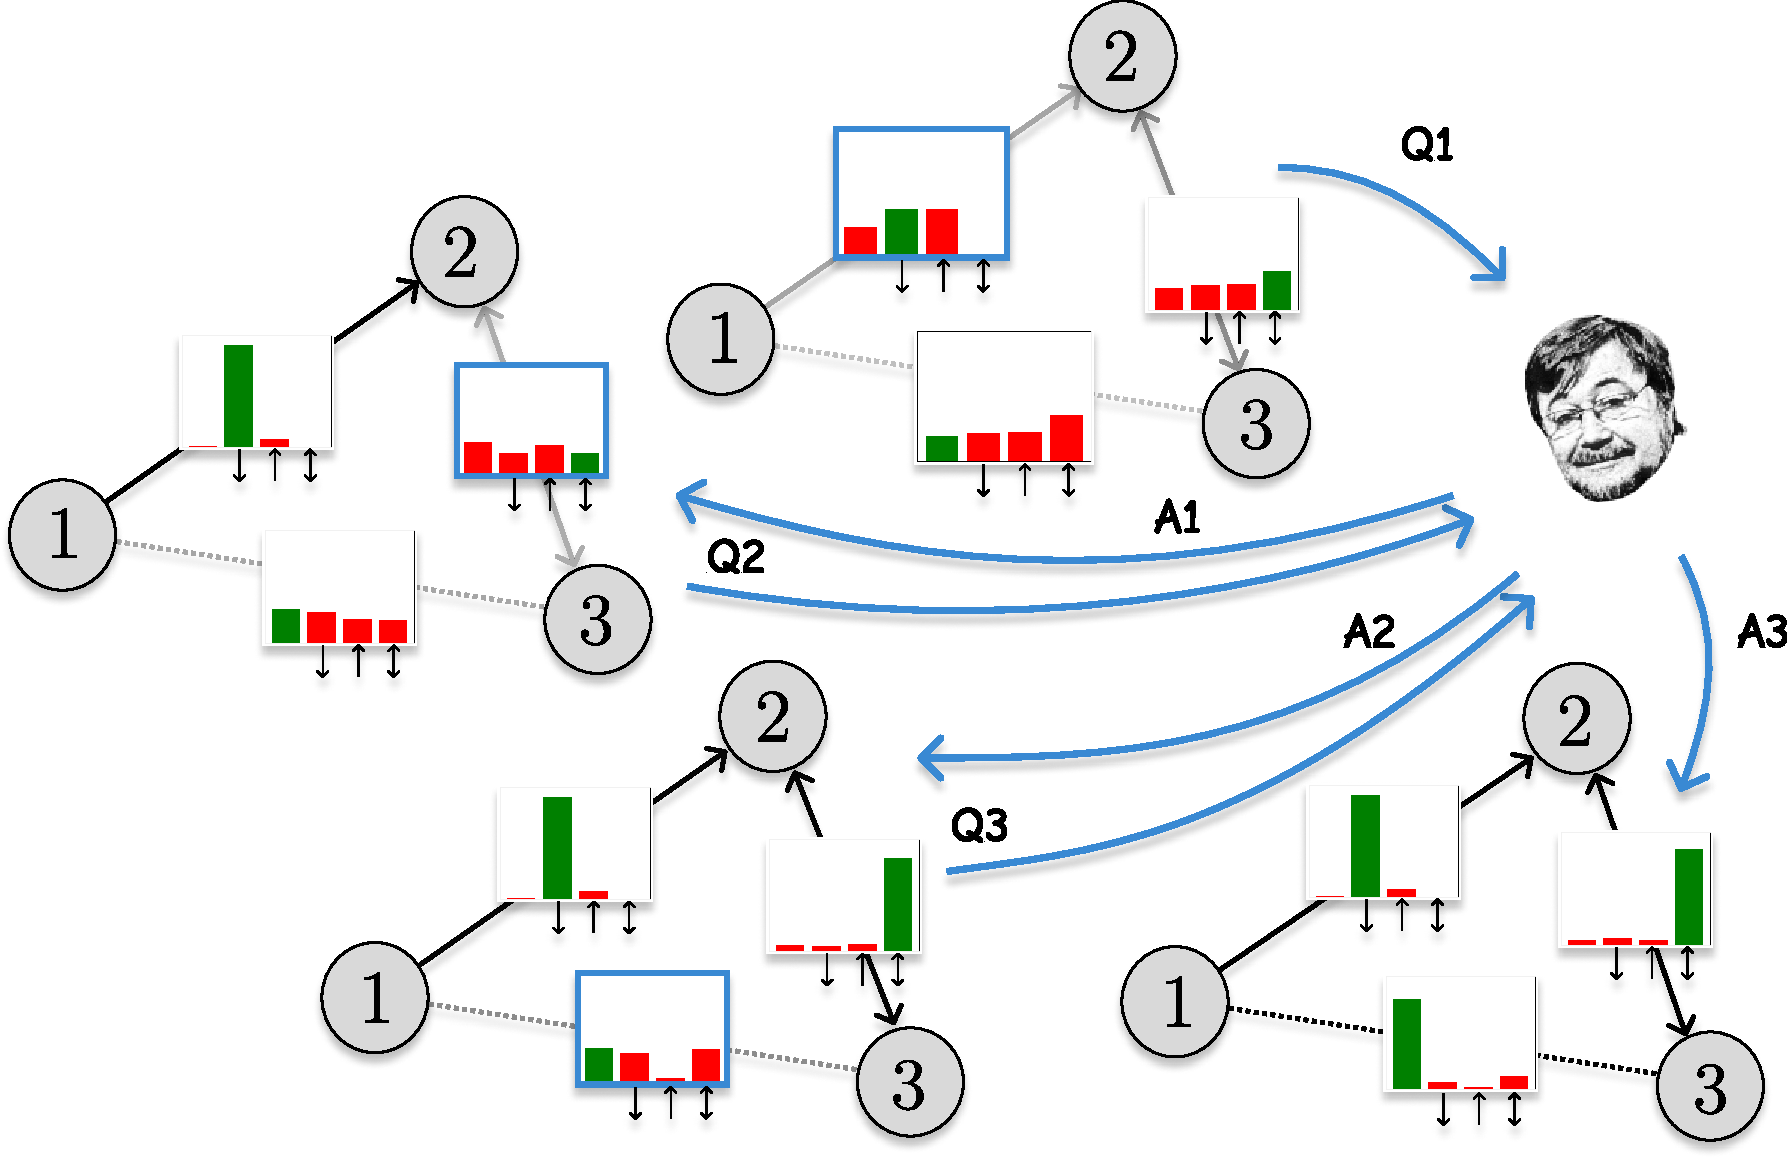
\includegraphics[width=\linewidth]{figures/hitl_judea_pearl_bw2.pdf} % vamos mandar um email pro pearl pedindo permissão dele? Podemos escrever amanhã :)
    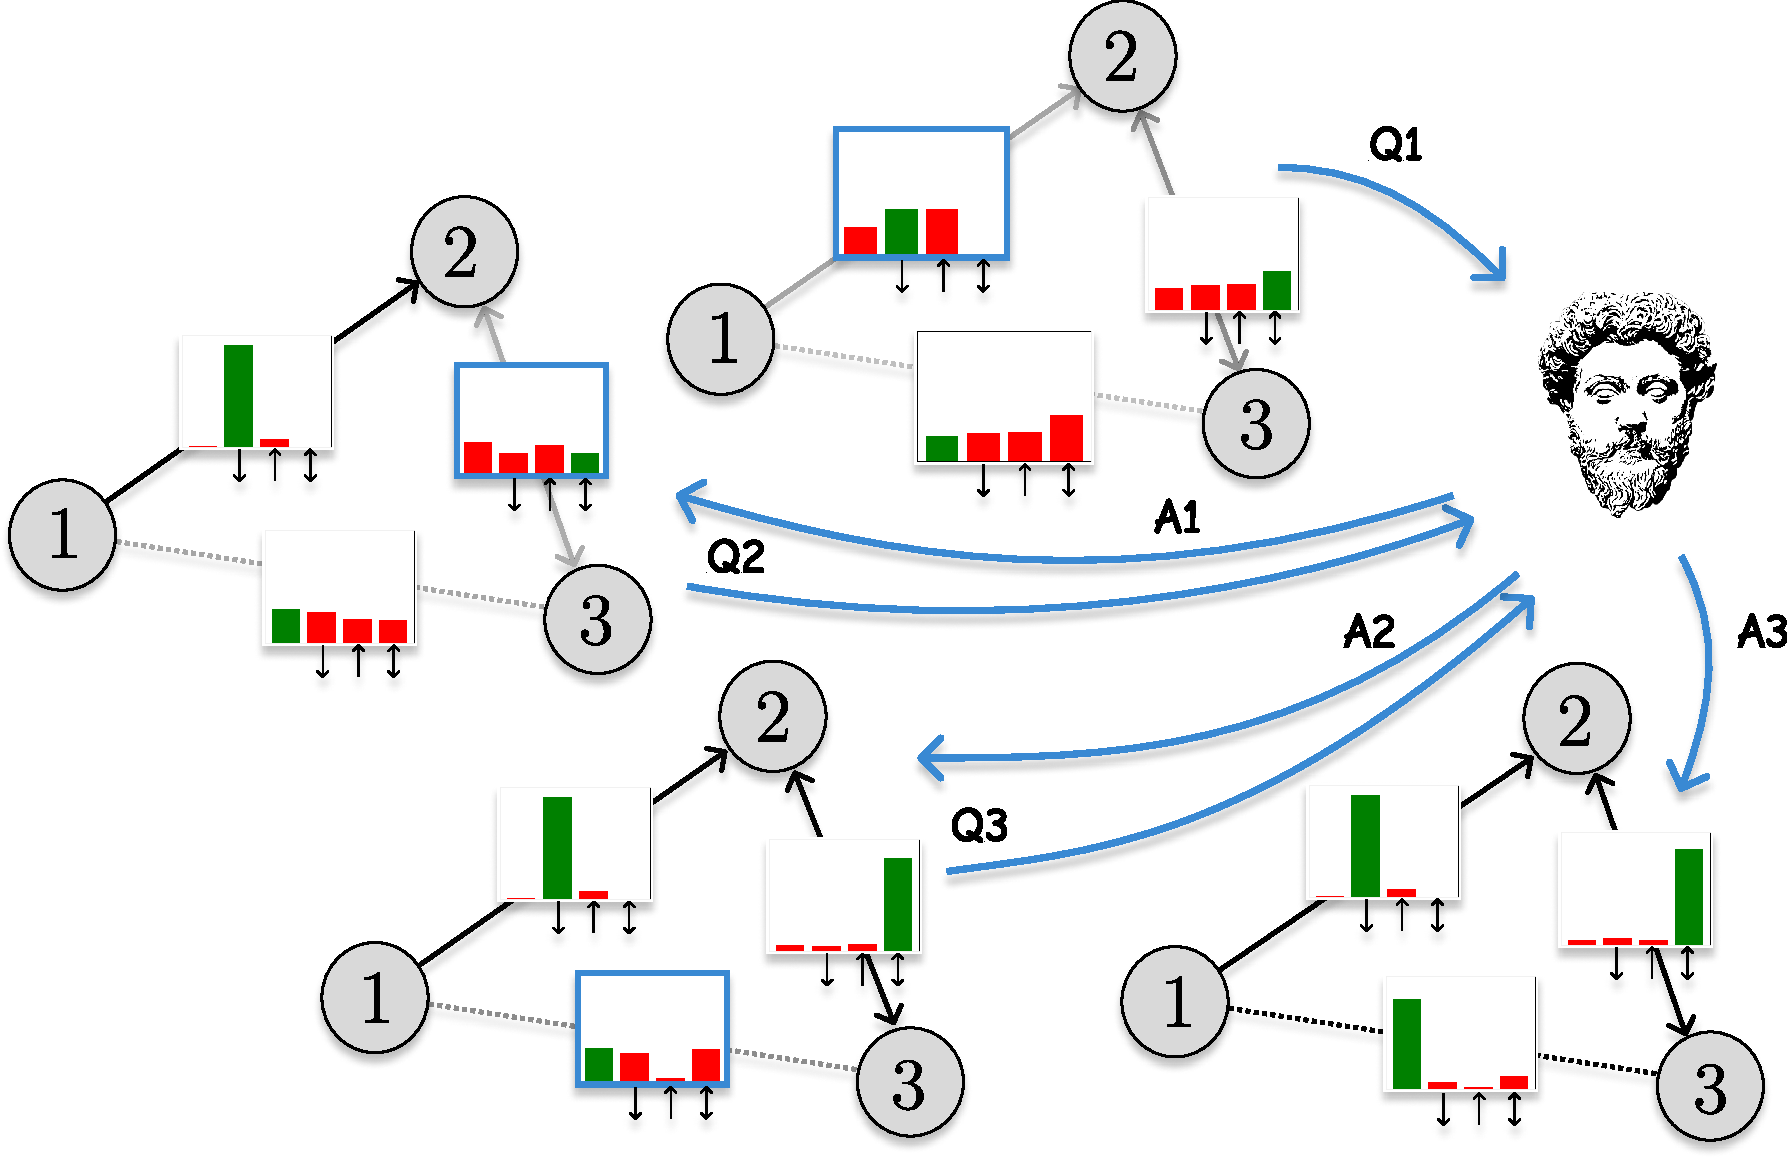
\includegraphics[width=0.7\linewidth]{figures/hitl_marcus_aurelius2.pdf} 
    \caption{\textbf{Human-in-the-loop probabilistic CD.} We first train an AGFN to fit a data-informed belief over AGs. Then, we iteratively refine it by 1) questioning (Q) experts on the relation between a highly informative pair of variables and 2) updating the belief given the potentially noisy answers (A). The histograms on top of the edges show marginals over edge types (green denotes ground truth). Notably, our belief increasingly concentrates on the true AG, $1 \rightarrow 2 \leftrightarrow 3$.
    }
    \label{fig:human}
\end{figure}

  
This work focuses on recovering the structure of the underlying causal diagram when unobserved confounders may be at play.
%
We propose to address this task by not only leveraging observational data but also by accounting for potentially noisy pieces of expert knowledge, otherwise unavailable as data. 
%
Throughout this work, we consider ancestral graphs (AGs) as surrogates for causal diagrams. AGs are particularly convenient since they encode latent confounding without explicitly invoking unobserved variables. Moreover, AGs capture all conditional independencies and ancestral relations among observed variables $\mathbf{V}$, as entailed by a causal diagram \citep{richardson2002ancestral}. 



%Importantly, AGs have emerged as an elegant and useful surrogate for causal diagrams in the presence of latent confounding. 
%They capture all conditional independence and ancestral relations among the observed variables $\mathbf{V}$, as entailed by the underlying causal model, without explicitly encoding the latent variables \citep{richardson2002ancestral}. 

 
In the realm of CD from solely observational data, algorithms aim to construct a compact representation of the joint observational distribution $P(\mathbf{V})$, which implies a factorization as a product of conditional probabilities. Notably, multiple models may entail the same conditional independencies; in such cases, they are denoted as Markov-equivalent. As a result, these algorithms can only reconstruct the class of Markov-equivalent models (AGs), denoted as the Markov Equivalence Class (MEC) and typically represented by a \textit{Partial Ancestral Graph} (PAG). Importantly, CD beyond the MEC by leveraging domain knowledge presents a critical challenge. Notably, there is no proper characterization of an equivalence class that accounts for knowledge stemming from both humans and data \citep{DBLP:conf/nips/WangQZ22}.

There is a variety of algorithms for CD from observational data, primarily categorized into constraint- and score-based methods. The former uses (in)dependence constraints derived via conditional independence tests to directly construct a PAG representing the MEC. The latter uses a goodness-of-fit score to navigate the space of AGs, selecting an optimum as a representative for the MEC. 

Nonetheless, methods within both paradigms suffer from unreliability when data is scarce. %.
%\cite{DBLP:journals/kbs/FarniaAC23}.  
Specifically, for the majority of the CD algorithms, formal assurances that the inferred MEC accurately represents the true causal model heavily rely on the so-called \textit{faithfulness} assumption, which posits that all conditional independencies satisfied by $P(\mathbf{V})$ are entailed by the true causal model \citep{zhang2016faces}. However, this presents a critical challenge in real-world scenarios, as violations of the faithfulness assumption become more prominent when relying on $P(\mathbf{V})$ estimated from limited data \cite{Uhler2012GeometryOT, andersen2013expect, DBLP:conf/uai/MarxGM21}. For constraint-based methods, hypothesis tests may lack the statistical power to detect conditional independencies accurately. These errors may propagate and trigger a chain reaction of erroneous orientations \cite{Zhang2008, zhalama2017heuristic, ng2021reliable}. For score-based methods, although score functions directly measure goodness-of-fit on observational data, small sample sizes can significantly skew the estimates for the population parameters. Consequently, structures deemed score-optimal may not necessarily align with the ground-truth MEC ~\cite{ogarrio2016gfci}. A major concern is that the overwhelming majority of CD algorithms produce a single representation of the MEC as output, without quantifying the uncertainty that arises during the learning process \cite{classen2012bccd, DBLP:conf/pkdd/JabbariRSC17}. This poses a significant challenge for experts, as it hinders their ability to validate the algorithm's outcome or gain insights into potential venues for improving inference quality.



To alleviate the lack of uncertainty quantification in CD, we propose sampling AGs from a %belief 
distribution defined using a score function, which places best-scoring AGs around the mode by design. This effectively provides end-users with samples that reflect the epistemic uncertainty inherent in CD, thus allowing their propagation through downstream causal inferences. In particular, we sample from our belief using \emph{Generative Flow Networks}  \citep[GFlowNets;][]{bengio2021GFlowNet,bengio2021GFlowNetfoundations}, 
which are generative models known for sampling diverse modes while avoiding the mixing time problem of MCMC methods, and not requiring handcrafted proposals nor accept-reject steps~\citep{bengio2021GFlowNet}.


Acknowledging the low-data regime as CD's primary challenge, we also propose actively integrating human feedback in the inferential process. This involves modeling user knowledge on the existence and nature (confounding/ancestral) of the relations and using it to weigh our beliefs over AGs. During our interactions with experts, we probe them about the relation of the pair of variables that optimizes a utility/acquisition function, for which we propose the negative expected cross-entropy between our prior and updated beliefs. %Compared to previous active elicitation strategies, 
Unlike prior strategies, 
our acquisition avoids the need to estimate the normalizing constant and predictive distribution of our updated belief, as needed for information gain and mutual information, respectively.
%our acquisition avoids approximating our updated belief's normalizing constant or the predictive distribution, as is the case for information gain and mutual information, respectively. 
Notably, we use importance sampling~\citep{marshall1954use, Geweke89}  to update our initial belief with the human feedback, which avoids retraining GFlowNets after each human interaction. 

While incorporating expert knowledge into CD has been a long-standing goal~\citep{DBLP:conf/uai/Meek95, DBLP:conf/nips/ChenSCD16,  DBLP:conf/pgm/LiB18, DBLP:conf/nips/WangQZ22}, existing works either rely on strong assumptions (e.g., causal sufficiency) or assume the knowledge is noiseless, aligned with the ground truth
~\citep{DBLP:conf/aistats/Andrews20, DBLP:conf/nips/WangQZ22}. 
Importantly, our work introduces the first iterative CD framework for AGs involving a human in the loop and accommodating potentially noisy feedback, as depicted in \Cref{fig:human}.

To validate our approach, we conduct experiments using the BIC score, for linear Gaussian causal models. Specifically, we assess: i) our ability to sample from score-based beliefs over AGs, ii) how our samples compare to samples from bootstrapped versions of state-of-the-art (SOTA) methods, and iii) the efficacy of our active knowledge elicitation framework using simulated humans. We observe that our method, Ancestral GFlowNet (AGFN), i) accurately samples from our beliefs over AGs; ii) consistently includes AGs with low structural error among its top-scored samples; and iii) is able to greatly improve performance metrics (i.e., SHD and BIC) when incorporating human in the loop. 



In summary, the \textbf{contributions} of our work are: 
\begin{enumerate}
    \item We leverage GFlowNets to introduce AGFN, the first CD algorithm for scenarios under latent confounding that employs fully-probabilistic inference on AGs;
    \item We show AGFN accurately learns distributions over AGs, 
    effectively capturing epistemic uncertainty.
    \item We propose an experimental design to query potentially noisy
     expert insights on relationships among pairs of variables that lead to optimal uncertainty reduction.
     \item We show how to incorporate expert feedback into AGFN without retraining them from scratch.
\end{enumerate}

\section{Background}\label{sec:background}
This section introduces the relevant notation and concepts. We use uppercase letters $V$ to represent a random variable or node in a graph, and boldface uppercase letters $\mathbf{V}$ to represent matrices or sets of random variables or nodes.

\vspace{2pt}
\noindent\textbf{Ancestral graphs. } Under the assumption of no selection bias, %In this work, where we assume causal systems without selection bias, we define 
an \textit{ancestral graph} (AG) $\mathcal{G}$ over $\mathbf{V}$ is a directed graph comprising directed ($\rightarrow$) and bidirected ($\leftrightarrow$) edges \cite{richardson2002ancestral,DBLP:conf/uai/Zhang07}. In any directed graph, if a sequence of directed edges, $V_i \rightarrow \cdots \rightarrow V_j$, connects two nodes $V_i$ and $V_j$, we refer to this sequence as a directed path. In this case, we also say that $V_i$ is an ancestor of $V_j$ and denote this relation as $V_i \in An(V_j)$. By definition, any AG $\mathcal{G}$ must further satisfy the following:
\begin{enumerate}
    \item there is no directed cycle, i.e., if $V_i \rightarrow V_j$ is in $\mathcal{G}$, then $V_j \not \in An(V_i)$; and
    \item there is no almost directed cycle, i.e., if $V_i \leftrightarrow V_j$  is in $\mathcal{G}$, then $V_j \not \in An(V_i)$ and $V_i \not \in An(V_j)$.
\end{enumerate}

As a probabilistic model, the nodes in an AG represent random variables, directed edges represent ancestral (causal) relationships, and bidirected edges represent associations solely due to latent confounding. 
For a complete characterization of AGs, refer to \citet{richardson2002ancestral}. 
%Importantly, AGs have emerged as an elegant and useful surrogate for causal diagrams in the presence of latent confounding. They capture all conditional independence and ancestral relations among the observed variables $\mathbf{V}$, as entailed by the underlying causal model, without explicitly encoding the latent variables \citep{richardson2002ancestral}. 

%In an AG, a path in which every node along it (except the endpoints) is a collider and every collider is an ancestor of an endpoint is termed as an inducing path \citep{DBLP:conf/uai/RantanenHJ21}. If an inducing path exists between two nodes $V_i$ and $V_j$ in an AG $\mathcal{G}$, then there is no set of other variables in $\mathcal{G}$ that can m-separate them. To uphold the pairwise Markov property (where each pair of non-adjacent vertices is m-separated by some set of other variables) in AGs, a common technical requirement is maximality. Formally, a \textit{maximal ancestral graph} (MAG) is defined as an AG with no inducing paths between non-adjacent variables \cite{richardson2002ancestral , DBLP:journals/jmlr/Zhang08}. %The MEC of AGs or MAGs is graphically represented by a PAG.
\vspace{2pt}

\noindent\textbf{Data generating model. } We assume that the data-generating model corresponds to a \emph{linear Gaussian structural causal model} (SCM) \citep{pearl:2k} defined by a 4-tuple $\mathcal{M} = \langle \mathbf{V}, \mathbf{U}, \mathcal{F}, P(\mathbf{U}) \rangle $, in which 
$\mathbf{V} = \{V_1, V_2, \dots, V_n\}$ is a set of $n$ observed random variables and $\mathbf{U} = \{U_1, U_2, \dots, U_n\}$ is the set of unobserved random variables. Further, let $Pa_i \subseteq \mathbf{V} \setminus \{V_i\}$ be the set of observed causes (parents) of $V_i$, and $U_i$ be the set of unobserved causes of $V_i$. Then, each structural equation $f_i \in \mathcal{F}$ is defined as: 
\begin{equation}
    V_i = \sum_{j: V_j \in Pa_i} \beta_{ij} V_j + U_i 
\end{equation}
with $P(\mathbf{U})$ being a multivariate Gaussian distribution with zero mean and a not necessarily identity covariance matrix $\boldsymbol{\Omega} = (\omega_{ij})_{1\leq i,j\leq n}$ --- the error terms $\{U_i\}$ are not necessarily mutually independent, implying that the system can be semi-Markovian (i.e., latent confounding may be present). 

Consider a lower triangular matrix of structure coefficients $\mathbf{B} = (\beta_{ij})_{1\leq i,j\leq n}$ such that $(\mathbf{I}-\mathbf{B})$ is invertible, and $\beta_{ij} \neq 0$ only if $V_j \in Pa_i$. Then, the set of structural equations is given in matrix form by 
\begin{equation}
\mathbf{V} = \mathbf{B} \mathbf{V} + \mathbf{U} \implies \mathbf{V} = (\mathbf{I}-\mathbf{B})^{-1} \mathbf{U}.
\end{equation}
%TODO falar que B e lower triangular and the model implies a covariance matrix 
The class of all linear Gaussian SCMs parametrized as \begin{equation}\label{eq:linear_model}
    \mathcal{N}_{\mathcal{M}}=\{ \mathcal{N}(\mathbf{0},\boldsymbol{\Sigma}) | \boldsymbol{\Sigma} = (\mathbf{I}-\mathbf{B})^{-1}\boldsymbol{\Omega} (\mathbf{I}-\mathbf{B})^{-\top}\}
\end{equation}
is represented by an AG in which, for every $i \neq j$, there is a directed edge $V_j \rightarrow V_i$ if $\beta_{ij} \neq 0$ and a bidirected edge $V_j \leftrightarrow V_i$ if $\omega_{ij} \neq 0$ \citep{richardson2002ancestral}.


% For a given observational dataset $\mathcal{D}$ and ancestral graph $\mathcal{G}$, maximum-likelihood estimates (MLE) of the parameters $\boldsymbol{\Theta} = (\mathbf{B}, \boldsymbol{\Omega})$
% %for a given set of observations and graph $\mathcal{M}
% can be calculated using the \textit{residual iterative conditional fitting (RICF)} algorithm \cite{DBLP:journals/jmlr/DrtonER09}. For a sample size $|\mathcal{D}| = m$, the corresponding log-likelihood is denoted by $l_{N}(\boldsymbol{\Theta})$.
\vspace{2pt}


\begin{figure}[t!]
    \centering
\adjustbox{scale=0.8}{
% https://q.uiver.app/#q=WzAsMTAsWzAsMywiR18wPVxce1xcfSJdLFsyLDAsIkdfMSA9IFxceyBYXzEgXFxyaWdodGFycm93IFhfMiBcXH0iXSxbMiwyLCJHXzIgPSBcXHsgWF8xIFxcbGVmdHJpZ2h0YXJyb3cgWF8yIFxcfSJdLFsyLDQsIkdfMyA9IFxceyBYXzEgXFxyaWdodGFycm93IFhfMyBcXH0iXSxbMiw2LCJHXzQgPSBcXHsgWF8yIFxccmlnaHRhcnJvdyBYXzMgXFx9Il0sWzQsMCwiR181ID0gXFx7IFhfMSBcXHJpZ2h0YXJyb3cgWF8yLCBYXzIgXFxyaWdodGFycm93IFhfMyBcXH0iXSxbNCw2LCJHXzcgPSBcXHsgWF8xIFxcbGVmdHJpZ2h0YXJyb3cgWF8yLCBYXzIgXFxyaWdodGFycm93IFhfMyBcXH0iXSxbNCwzLCJHXzYgPSBcXHsgWF8xIFxcbGVmdHJpZ2h0YXJyb3cgWF8yLCBYXzEgXFxyaWdodGFycm93IFhfMyBcXH0gIl0sWzYsM10sWzcsM10sWzAsMV0sWzAsMl0sWzAsM10sWzAsNF0sWzEsNV0sWzQsNl0sWzQsNV0sWzIsNl0sWzIsN10sWzMsN10sWzUsOCwiUihHXzYpIiwyXSxbNyw4LCJSKEdfNykiLDJdLFs2LDgsIlIoR183KSIsMl0sWzIxLDksIiIsMix7ImxldmVsIjoxLCJzdHlsZSI6eyJuYW1lIjoiYWRqdW5jdGlvbiJ9fV1d
\begin{tikzcd}[sep=small]
	&& {\mathcal{G}_1 = \{ X_1 \rightarrow X_2 \}} && {\mathcal{G}_5 = \{ X_1 \rightarrow X_2, X_2 \rightarrow X_3 \}} \\
	\\
	&& {\mathcal{G}_2 = \{ X_1 \leftrightarrow X_2 \}} \\
	{\mathcal{G}_0=\{\}} &&&& {\mathcal{G}_6 = \{ X_1 \leftrightarrow X_2, X_1 \rightarrow X_3 \} } &&&& {	\square} \\
	&& {\mathcal{G}_3 = \{ X_1 \rightarrow X_3 \}} \\
	\\
	&& {\mathcal{G}_4 = \{ X_2 \rightarrow X_3 \}} && {\mathcal{G}_7 = \{ X_1 \leftrightarrow X_2, X_2 \rightarrow X_3 \}}
        \arrow[from=4-1, bend left=5, dashed, -stealth, opacity=0.7,color=gray, to=4-9]
        \arrow[from=5-3, dashed, bend right=10, -stealth, opacity=0.7,color=gray, to=4-9]
        \arrow[from=3-3, bend left=10, dashed, -stealth, opacity=0.7,color=gray,  crossing over, to=4-9]
        \arrow[from=1-3, bend left=10, dashed, -stealth, opacity=0.7,color=gray,  crossing over, to=4-9]
        \arrow[from=7-3, controls={+(3.0,-0.3) and +(-0.5,-1.5)}, dashed, -stealth, opacity=0.7,color=gray, to=4-9]
	\arrow[from=4-1, bend left=20, very thick, -stealth, opacity=1,color=blue, to=1-3]
	\arrow[from=4-1, bend left=10, very thick, -stealth, opacity=1,color=green!50!blue, to=3-3]
	\arrow[from=4-1, bend right=10, very thick, -stealth, opacity=1,color=yellow!50!red, to=5-3]
	\arrow[from=4-1, bend right=20, very thick, -stealth, opacity=1,color=red, to=7-3]
	\arrow[from=1-3, very thick, -stealth, opacity=1,color=blue, to=1-5]
	\arrow[from=7-3, very thick, -stealth, opacity=0.5,color=red, to=7-5]
	\arrow[from=7-3, very thick, -stealth, opacity=0.5,color=red, crossing over, controls={+(2,0.5) and +(7,-4)}, to=1-5]
	\arrow[from=3-3, bend left=10, very thick, -stealth, opacity=0.8,color=green!50!blue,  crossing over, to=7-5]
	\arrow[from=3-3, bend left=10, very thick, -stealth, opacity=0.7,color=green!50!blue,  to=4-5]
	\arrow[from=5-3, bend right=10, very thick, -stealth, opacity=1,color=yellow!50!red, crossing over, to=4-5]
	\arrow["{R(\mathcal{G}_5)}" description, bend left=20, very thick, -stealth, opacity=1,color=blue!50!red, from=1-5, to=4-9]
	\arrow["{R(\mathcal{G}_6)}" description, very thick, -stealth, opacity=1,color=yellow!90!blue!50!green!50!red, crossing over, from=4-5, to=4-9]
	\arrow["{R(\mathcal{G}_7)}" description, very thick, -stealth, opacity=1,color=blue!50!green!40!red!70, bend right=20, from=7-5, to=4-9]
\end{tikzcd}}
    \caption{\textbf{Illustration of the generative process of AGs} $\{\mathcal{G}_5, \mathcal{G}_6, \mathcal{G}_7\}$ using GFlowNets. Starting with an empty graph $\mathcal{G}_0$, we add edges between variables $\{X_1, X_2, X_3\}$ according to the action-policy $\pi_F$. Solid edges trace trajectories leading to sampled graphs. Dashed lines represent non-realized transitions to terminal state $\square$.}
    \label{fig:ancgfn}
\end{figure}
\noindent\textbf{GFlowNets.}
Generative Flow Networks \citep[GFlowNet;][]{bengio2021GFlowNet, bengio2021GFlowNetfoundations} are generative models designed to sample from a finite domain $\mathcal{X}$ proportionally to some reward function $R:\mathcal{X}\rightarrow\mathbb{R}_{+}$, which may be parametrized using neural networks. In this work, we define $R$ as a strictly decreasing transformation of the BIC (more details in \cref{sec:ancestralGFlowNet}).
GFlowNets also assume there is a compositional nature to the elements $x \in \mathcal{X}$, meaning that they can be built by iteratively acting to modify a base object (i.e., an \emph{initial state}). For instance, graphs can be built by adding edges to a node skeleton \citep{deleu2022bayesian} or molecules by adding atoms to an initial structure \citep{bengio2021GFlowNet}. 

%Cut to sampling as network flow on the pointed DAG?

%More specifically, starting from an initial state $s_0$ and setting $i=0$, we take action $a \in \mathcal{A}_{s_i}$ with probability 

The generative process follows a trajectory of states $s\in\mathcal S$ guided by a transition probability $\pi_{F}:\mathcal{S}^2\rightarrow [0,1]$. In turn, $\pi_F$ is proportional to a \emph{foward flow} function $F_{\theta} : \mathcal{S}^2\rightarrow \mathbb{R}_{+}$, which is parameterized by a neural network $\theta$. Let $\text{Pa}(s')$ ($\text{Ch}(s')$) be the set of all states which can transition into (directly reached from) $s'$. Then, $\pi_F$ is defined as
\begin{equation}
\pi_F(s'|s) = \frac{F_{\theta}(s\rightarrow s')}{\sum_{{s'\in \text{Ch}(s)}} F_{\theta}(s\rightarrow s')}. 
\end{equation} 

The support $\mathcal{X}$ of $R$ is contained within $\mathcal{S}$. There are also two special states in $\mathcal{S}$: an \emph{initial state} $s_0$ and a \emph{terminal state} $s_f$. We start with the initial state $s_0$ and transform it to a new valid state $s$ with probability $\pi_F(s|s_0;\theta)$.
We keep iterating this procedure until reaching $s_f$. States $s$ valid as final samples ($s\in\mathcal X$) are known as \textit{terminating states} and have a positive probability for the transition $s\rightarrow s_f$. \Cref{fig:ancgfn} illustrates this process with $\mathcal{X}$ being the space of AGs.
%
Crucially, the same parameterization $\theta$ is used for all transition probabilities $\pi_F(\cdot|s;\theta)$ given any departing state $s$, allowing for generalization to states never visited during training. 

% This procedure induces a Markov Decision Process. 
As the GFlowNet framework requires that no sequence of actions leads to a loop, we represent the space of possible action sequences by a pointed Directed Acyclic Graph (DAG)~\citep{bengio2021GFlowNetfoundations}. The generation of any sample $x \in \mathcal{X}$ follows a trajectory $\tau=(s_0, s_1, \ldots, s_{T} = x, s_f) \in \mathcal S^{T+2}$ for a $T\geq0$. Different trajectories may lead to the same sample $x$. 
%
To ensure we sample proportionally to $R$, we search for a GFlowNet that satisfies the \emph{flow-matching condition}, i.e., $\forall s'\in\mathcal{S}$: 
\begin{equation}
    \sum_{s\in\text{Pa}(s')} F_\theta(s\rightarrow s') = R(s') + \sum_{s''\in \text{Ch}(s')}F_\theta(s'\rightarrow s'').
    \label{eq:balance}
\end{equation} 

\Cref{eq:balance} implies the flow that enters $s^\prime$ equals the flow leaving $s^\prime$, except for some flow $R(s')$ leaking from $s^\prime$ into $s_f$. We let $R(s) = 0$ for $s \notin \mathcal{X}$. Eventually, it may be that all states $s$ are valid candidates, i.e., $\mathcal{S} = \mathcal{X} \cup \{s_{f}\}$. If so, each of  \cref{eq:balance}'s solutions satisfies a \textit{detailed-balance condition}, 
\begin{equation} \label{eq:dbalance} 
    \frac{R(s) F_{\theta}(s \rightarrow s') F_{\theta}(s' \rightarrow s_{f})}{F_{\theta}(s \rightarrow s_{f})} = R(s') F_{B, \theta}(s' \rightarrow s), 
\end{equation}
for a parametrized backward flow $F_{B, \theta} \colon \mathcal{S}^{2} \rightarrow \mathbb{R}_{+}$ \cite{deleu2022bayesian}. In practice, we enforce \cref{eq:dbalance} by minimizing
\begin{equation} \label{eq:dbalancetheta} 
\mathcal{L}(\theta) \! = \!\underset{s \rightarrow s^\prime}{\mathbb{E}}\!\left[\!\left(\! \log \frac{R(s') \pi_{F_B}(s | s^\prime; \theta) \pi_{F}(s_{f} | s; \theta)}{R(s) \pi_{F}(s^\prime | s; \theta) \pi_{F}(s_{f} | s^\prime; \theta)} \!\right)^{2} \!\right].
\end{equation} 
% for a distribution $\upsilon$ fully-supported on the transitions $s \rightarrow s'$. 
% All intermediate states, including $s_0$, will be valid ancestral graphs in this work. Therefore, we will have $\mathcal{X} \cup \{s_f\} = \mathcal{S}$.

% Others, such as molecule discovery, may require temporarily traversing states $s\in \mathcal S\setminus \mathcal X$, which are not valid final samples \cite{bengio2021GFlowNet} --- these may correspond, for instance, to an invalid configuration of atoms, before arriving at a final $s\in \mathcal X$ which will be sampled. 
%


%Beginning in $s_0$, a stochastic action policy $\pi_F( \cdot | s_t ; \theta)$ selects an action for each step $t$ until reaching $s_f$, with probability proportional to a function $F_\theta(s\rightarrow s') : \mathcal S^2\rightarrow \mathbb R_{\geq 0}$ named \textit{forward flow}.




\section{Ancestral GFlowNets}
\label{sec:ancestralGFlowNet}

We propose AGFN, a GFlowNet-based method for sampling AGs using a score function. Specifically, AGFN encompasses a GFlowNet with the following characteristics:

\begin{enumerate}
    \item Each trajectory state is a valid AG $\mathcal{G}_t$.
    \item A terminating state's reward $R(\mathcal{G_T})$ is a score-based potential suitable for CD of AGs.
    \item A well-trained AGFN samples AGs with frequencies proportional to their rewards and with the best-scoring AG being, by design, the mode.
\end{enumerate}

The generation of a trajectory $\tau = \{\{\}, \mathcal{G}_1, \mathcal{G}_2, \ldots, \mathcal{G}_T \}$ begins with a totally disconnected graph with nodes $\mathbf{V}$, iteratively adding edges of types $\{\leftarrow, \rightarrow, \leftrightarrow\}$ between pairs of variables. 
%
%The growing trajectory adheres to ancestral constraints in \cref{eq:cond:ancestral} and does not add edges with identical endpoints. 
%
The following paragraphs describe AGFN. For further details, please refer to the Appendix.


\vspace{2pt}

\noindent\textbf{Action constraints.} To ensure AGFN only samples AGs, we mask out actions that would lead to paths forming cycles or almost cycles. To achieve this, we verify whether the resulting graph respects \citet{bhattacharya2021differentiable}'s algebraic characterization of the space of AGs. 
%
More specifically, any AG $\mathcal{G}$ is characterized by an adjacency matrix $\mathbf{A}_d \in \mathbb{R}^{n \times n}$ for its directed edges and another adjacency matrix $\mathbf{A}_b \in \mathbb{R}^{n \times n}$ for its bidirected edges, adhering to:
\begin{equation} \label{eq:cond:ancestral} 
    \text{trace}(\exp\{ \mathbf{A}_d \}) - n + \mathbf{1}^{T}(\exp\{ \mathbf{A}_d \} \odot \mathbf{A}_b)\mathbf{1} = 0,  
\end{equation}
in which $\mathbf{1}$ is a $n$-dimensional unit vector and  $\odot$ denotes the Hadamard (elementwise) product of matrices. 

\noindent\textbf{Score-based belief.}  We propose using a strictly decreasing transformation of a score function $U$ as the reward $R$ for AGFN. More precisely, we define $R$ as 
\begin{equation}\label{eq:reward}
    R(\mathcal{G}) = \exp\left\{\frac{\mu - U(\mathcal{G})}{\sigma}\right\} 
\end{equation}
for given constants $\mu\in\mathbb{R}$ and $\sigma \in \mathbb{R}^+$ that ensure numerical stability~\citep{zhang2023robust}. In practice, we sample $S$ AGs $\{\mathcal{G}^{(s)}\}_{s=1}^{S}$ from an untrained AGFN, and set $\mu = \nicefrac{1}{S} \sum_s U(\mathcal{G}^{(s)})$ and $\sigma = \sqrt{\nicefrac{1}{S} \sum_s (U(\mathcal{G}^{(s)}) - \mu)^2}$.
\vspace{2pt}

\noindent\textbf{Score for linear Gaussian models.} Since we focus on linear Gaussian models, we choose the \textit{extended Bayesian Information Criterion} \cite{DBLP:conf/nips/FoygelD10} as our score function. Specifically, for any AG $\mathcal{G}=(\mathbf{V}, \mathbf{E})$: 
\begin{align} \label{eq:bic} 
    U(\mathcal{G}) &= - 2 l_{N}(\hat{\mathbf{B}}, \hat{\boldsymbol{\Omega}}) + |\mathbf{E}| \log n + 2 |\mathbf{E} | \log |\mathbf{V}|, % .
\end{align}
in which $(\hat{\mathbf{B}}, \hat{\boldsymbol{\Omega}})$ is the  MLE estimate of  model parameters (see \cref{eq:linear_model}) obtained using the \emph{residual iterative conditional fitting} algorithm \cite{JMLR:v10:drton09a}.
\vspace{4pt}



\noindent\textbf{Forward flow.} We use a Graph Isomorphism Network (GIN) \cite{DBLP:conf/iclr/XuHLJ19} $\Phi$ to compute a $d$-dimensional representation for each node in the AG $\mathcal{G}_{t}$ at the $t$-th step of the generative process and use sum pooling to get an embedding for $\mathcal{G}_t$. Then, considering $\mathcal{A}_{t}$ as the space of feasible actions at $\mathcal{G}_t$ (i.e., those leading to an AG),  we use an MLP $\phi \colon \mathbb{R}^{d} \rightarrow \mathbb{R}^{|\mathcal{A}_{t}|}$ with a softmax activation at its last layer to map $\mathcal{G}_t$'s embedding to a distribution over $\mathcal{A}_{t}$. More precisely, given $\mathbf{H}^{(t)} = \Phi(\mathcal{G}_{t}) \in \mathbb{R}^{|\mathbf{V}| \times d}$, we compute 
\begin{equation}
    \mathbf{p} = \phi\left(\sum_{v \in \mathbf{V}} \mathbf{H}_{v}^{(t)} \right) 
\end{equation}
as the probability distribution over the feasible actions at $\mathcal{G}_{t}$.


% During training, we sample an action $a \sim \text{Cat}(0.5 \cdot \mathbf{p} + 0.5 \cdot |\mathcal{A}_{n}|^{-1})$ from a mixture between the $\mathbf{p}$ and uniform distribution over $\mathcal{A}_{n}$ to ensure that the GFlowNet doesn't get stuck anywhere. Otherwise, we sample $a \sim \text{Cat}(\mathbf{p})$.  

% We use a Graph Isomorphism Network (GIN) $\Phi$ to compute a $d$-dimensional representation for each variable of the graph $\mathcal{G}_t$ at stage $t$, projected to action-probabilities using MLPs $\Psi^{(1)} \colon \mathbb{R}^{2d} \rightarrow \mathbb{R}$, $\Psi^{(2)} \colon \mathbb{R}^{d} \rightarrow \mathbb{R}$, and $\Psi^{(3)} \colon \mathbb{R}^{d} \rightarrow \mathbb{R}$. 
% Specifically, let $\mathbf{h}^t = \Phi(\mathcal{G}_t) \in \mathrm{R}^{|\mathbf{V}| \times d}$ be the embedding matrix of $\mathcal{G}_t$. For directed edge $e = (v, u)$, define $\mathbf{y}_{(u, v)}$; for bidirected edge $e = \{u, v\}$, define $\mathbf{y}_{\{u, v\}}$; and for state graph $\mathcal{G}_t$, define $\mathbf{y}_{t}$.
% Let $\mathbf{y}$ concatenate $\mathbf{y}_{(u, v)}$, $\mathbf{y}_{\{u, v\}}$, and $\mathbf{y}_{t}$. The transition probability from graph $\mathcal{G}_t$ to $\mathcal{G}_{t+1}$ through the action of adding an edge is $P_{\theta}( \mathcal{G}_{t+1} | \mathcal{G}_t) = \texttt{Softmax}(\tilde{\mathbf{y}})$, with $\tilde{\mathbf{y}} = \mathbf{m} \odot \mathbf{y} + \epsilon \cdot (1 - \mathbf{m})$, with $\epsilon = -10^{5}$ and binary mask of allowed edges additions $\mathbf{m}$.
% \begin{align}
%     \mathbf{y}_{(u, v)} &= \Psi^{(1)} (\mathbf{H}_{u}^t \oplus \mathbf{H}_{v}^t) \in \mathbb{R}^{2d} \label{eq:directed_e} \\
%     \mathbf{y}_{\{u, v\}} &= \Psi^{(2)} (\mathbf{H}_{u}^t + \mathbf{H}_{v}^t) \label{eq:bidirected_e} \\
%     \mathbf{y}_{t} &= \Psi^{(3)}\left(\frac{1}{|\mathbf{V}|} \sum_{u \in \mathbf{V}} \mathbf{H}_{u}^t\right) \label{eq:fullgraph_e}
% \end{align}

%\noindent\textbf{Backward Flow.} Backward actions consist of edge removals. We use an MLP that maps the flattened adjacency matrices of $\mathcal{G}_{t}$ into a probability distribution of feasible backward actions at $\mathcal{G}_{t}$ (i.e., the actions corresponding to existing edges). Remarkably, using a backward flow ensures the uniqueness of the solution to the flow-matching problem in \cref{eq:dbalance} and reduces the search space of the optimization problem tackled during training \cite{bengio2021GFlowNetfoundations}. 
\noindent\textbf{Backward flow.} Backward actions correspond to removing edges. Following \citet{shen2023towards}, we parametrize the backward flow $F_B$ with an MLP and alternate between updating $\pi_F$ and $\pi_{F_B}$, using gradient-based optimization.

% the flattened adjacency $\mathbf{A}_t$ to log probabilities for possible backward transitions $\mathbf{y}_b^t=\Phi_{b}(\mathbf{A}_t)$. The transition probability from $\mathcal{G}_t$ to $\mathcal{G}_{t-1}$ through removal of an edge is $P^F_{\theta}(  
% \mathcal{G}_{t-1} | \mathcal{G}_{t}) = \texttt{Softmax}(\tilde{\mathbf{y}})_{a}$, with $\tilde{\mathbf{y}} = \mathbf{m}^{(b)} \odot \mathbf{y}_b^t + \epsilon \cdot (1 - \mathbf{m}^{(b)})$, with $\epsilon = -10^{5}$ and binary mask of allowed edges removals $\mathbf{m}^{(b)}$.
\vspace{1pt}


% Firstly, we use an untrained policy to exploratorily navigate within the space of this

% Training involves two stages: (1) exploratory navigation to estimate $\mu$ and $\sigma$ of $U(\mathcal{G})$ and (2) target density adjustment using Equation~\eqref{eq:reward} to minimize the \textit{detailed balance loss $\mathcal{L}_{\text{DB}}$ }\cite{deleu2022bayesian}.


% \noindent\textbf{Preprocessing.} 

% Inference over the energy-based distribution $p(\mathcal{G}) \propto \exp\{-U(\mathcal{G}) / T\}$ on ancestral graphs uses the extended BIC \cite{DBLP:conf/nips/FoygelD10} potential function $U(\mathcal{G})$. Training maximizes this criterion, estimating parameters $\boldsymbol{\Theta} = (\mathbf{B}, \boldsymbol{\Omega})$.
% \vspace{2pt}

\section{Human-in-the-Loop Causal Discovery}
\label{sec:hitl}



Concluding the training, we propose leveraging the AGFN-generated samples to design questions for the expert that optimize the reduction of entropy in the distribution $p_{\theta}(\mathcal{G})$ over the space of AGs. Then, we %collect human feedback, 
use the human feedback to update $p_\theta(\mathcal{G})$, and iteratively repeat the process. The following paragraphs describe %, in that order, 
i) how we model human feedback, ii) how we update our belief over AGs given human responses, and iii) our experimental design strategy for expert inquiry.
\vspace{2pt}

\subsubsection{Modeling human feedback.} We assume humans are capable of answering questions regarding the ancestral relationship between pairs of random variables. In this case, we model their prior knowledge on a relation $r=\{U, V\}$ between nodes $U, V \in \mathbf{V}$ as a categorical distribution over a random variable denoted $\omega_{r}$. Fix an arbitrary total order $<$ in $\mathbf{V}$. By definition, $\omega_r=1$ if there is no edge between $U$ and $V$; 
$\omega_{r} = 2$ if $U$ is ancestor of $V < U$; $\omega_{r} = 3$ if $V$ is ancestor of $U > V$; and $\omega_{r} = 4$ if there is a bidirected edge between $U$ and $V$. Since the human has access to our AGFN before being probed for the first time, we set $\rho_{r, k} = p_{\theta}(\omega_r=k)$ as the prior probability of $\omega_r=k$. Moreover, we consider that the expert's feedback $f_{r} \in \{1, 2, 3, 4\}$ on the relation $r$ is a noisy realization of the true, unobserved value of the relation feature $\omega_{r}$ under the expert's model. Putting all elements together results in a two-level Bayesian hierarchical scheme for categorical data:
\begin{alignat}{2}
    \omega_{r} &\sim \text{Cat}(\boldsymbol{\rho}_{r}), \\
    f_{r} | \omega_{r} &\sim \text{Cat}\left(\delta_{\omega_{r}} \cdot \pi + (\mathbf{1} - \delta_{\omega_{r}}) \cdot \left( \frac{1 - \pi}{3} \right) \right), 
\end{alignat}
in which $\boldsymbol{\rho}_{r} = (\rho_{r, 1}, \rho_{r, 2}, \rho_{r, 3}, \rho_{r, 4})$ represents our prior beliefs about the relations' features, $\pi \in [0, 1]$ reflects the reliability of the expert's feedback, and $\delta_{k}$ is the $k$-th canonical basis of $\mathbb{R}^4$. Conveniently, the posterior distribution of the relation feature $\omega_{r}$ given the feedback $f_{r}$ is a categorical distribution parametrized by  
\begin{equation}
    \frac{\boldsymbol{\rho}_{r}}{\eta_{r}} \odot \left( \pi \cdot \delta_{f_{r}} + \left(\frac{1 - \pi}{3}\right) \cdot (\mathbf{1} - \delta_{f_{r}})\right), % . 
\end{equation}
with $\eta_{r} = \rho_{r, f_{r}} \cdot \pi + \left(\frac{1 - \pi}{3}\right) \cdot (1 - \rho_{r, f_{r}})$.  
\vspace{2pt}

\begin{figure*}[!t] 
    \centering
    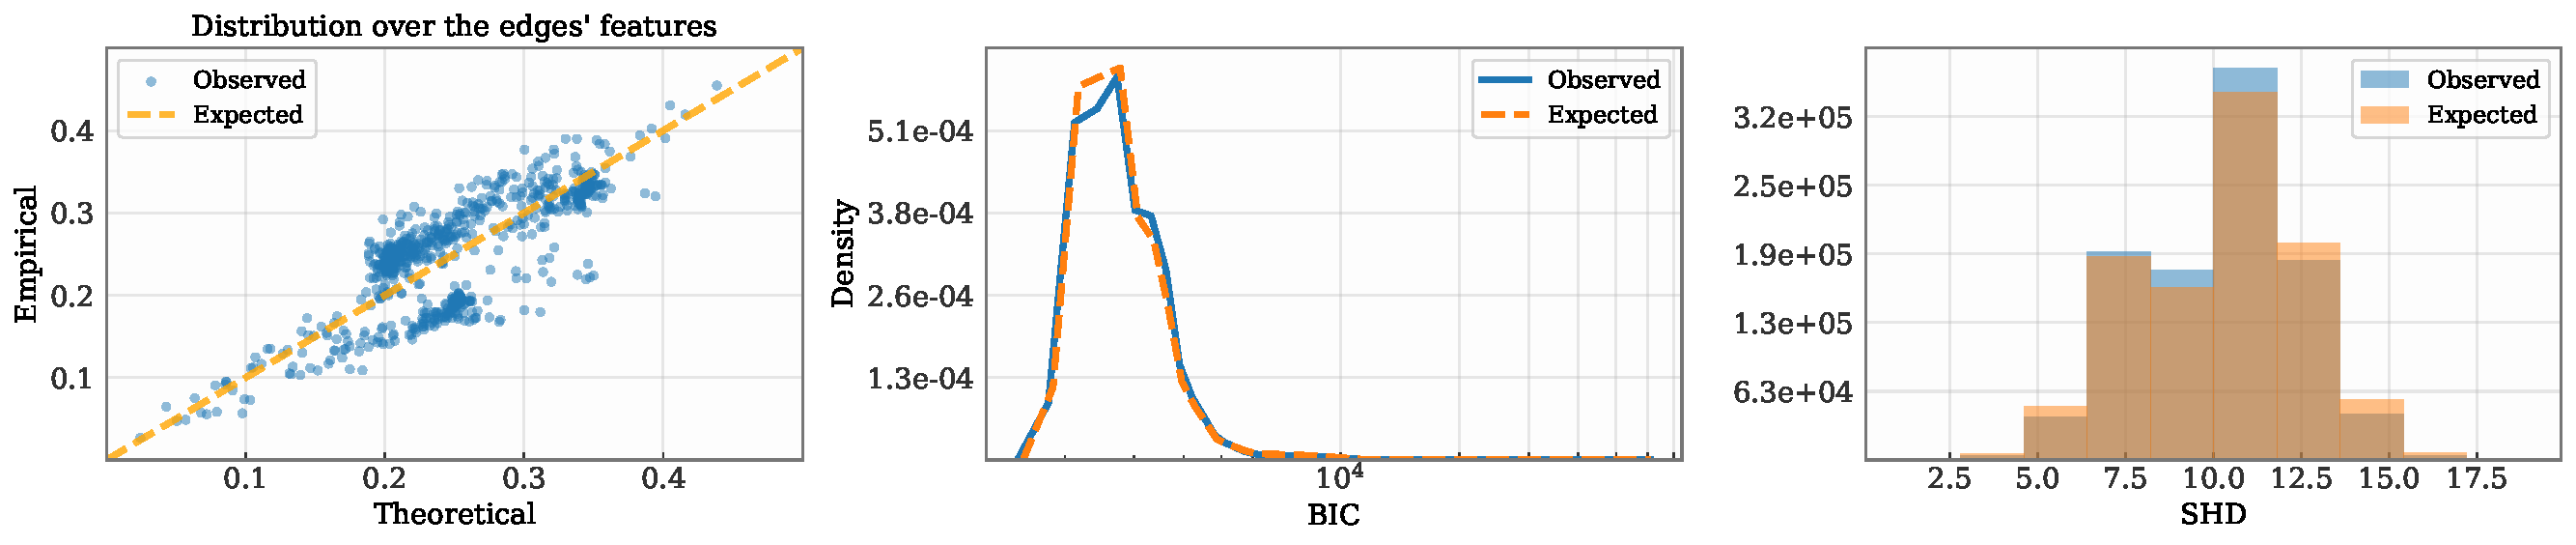
\includegraphics[width=\linewidth]{figures/expected_observed.pdf}
    \caption{\textbf{Sampling quality.} The reward-induced marginal distribution over graph features is adequately approximated by the marginal distribution learned by the GFlowNet.}
    \label{fig:distribution}
\end{figure*}

\subsubsection{Updating beliefs.} We update our AGFN by weighing it by our posterior over the expert's knowledge, described in the previous paragraph, similarly to a product-of-experts approach \cite{Hinton2002}. For this, let $\mathbf{f}_{K} = (f_{r_{k}})_{1 \le k \le K}$ be the sequence of $K$ feedbacks issued by the expert and define our novel belief distribution $q(\mathcal{G}; \mathbf{f}_{K})$ over the space of AGs as 
\begin{equation}
    q(\mathcal{G} ; \mathbf{f}_{K}) \propto p_{\theta}(\mathcal{G}) \prod_{1 \le k \le K} p(\omega_{r_{k}} | f_{r_{k}}). 
\end{equation}
Importantly, we use $p_{\theta}$ as proposal distribution in importance (re-)sampling \cite{gordon1993novel} to approximately sample from $q(\mathcal{G}; \mathbf{f}_{K})$ --- or to approximate the expected value of a test function. More precisely, we estimate the value of a function $h$ over the space of AGs as:
\begin{equation}\label{eq:resample}
    \mathbb{E}_{q}[h(\mathcal{G})] \approx \sum_{t=1}^{T} c^{-1} \frac{q(\mathcal{G}^{(t)} ; \mathbf{f}_{K})}{p_{\theta}(\mathcal{G}^{(t)})} h(\mathcal{G}^{(t)})
\end{equation}
with $(\mathcal{G}^{(t)})_{t=1}^T \sim p_\theta(\mathcal{G})$ and $ c = \sum_{t=1}^T\nicefrac{q(\mathcal{G}^{(t)}; \mathbf{f}_{K})}{p_{\theta}(\mathcal{G}^{(t)})}$.
\vspace{2pt}


\subsubsection{Active knowledge elicitation.} To make the most out of possibly costly human interactions, we query the human about the relation that maximally reduces the expected cross-entropy between our belief over AGs before and after human feedback. More precisely, we define an acquisition function $a_k : {{\mathbf{V}}\choose{2}} \rightarrow \mathbb{R}$ for the $k>1$-th inquiry as:
\begin{equation} \label{eq:divergence} 
    a_{k}(r) = - \mathbb{E}_{f_r \sim p(\cdot| \mathbf{f}_{K})}\big[ \mathbf{H} \left( q(\mathcal{G}; \mathbf{f}_{K}, f_r), q(\mathcal{G} ; \mathbf{f}_{K} ) \right) \! \big] 
\end{equation}
in which $p(f_r|\mathbf{f}_{K})$ is the posterior predictive distribution according to the user model, $q_0 \propto R$ and $\mathbf{H}(\cdot, \cdot)$ is the cross-entropy. Then, we maximize this acquisition to select which relation $\tilde{r}_k$ we will probe the expert, i.e.: 
\begin{equation}
    \tilde{r}_k = \argmax_{r \in {{\mathbf{V}}\choose{2}}} a_{k}(r). % . 
\end{equation}

As aforementioned, we use importance sampling with $q_0$ as a proposal to estimate the acquisition function $a_k$. This allows us to leverage AGFN samples and effectively avoid the need for retraining them. 
%
It is worth mentioning that because $\mathbf{H}(p, p^\prime) \geq \mathbf{H}(p, p)$ for any two distributions $p$ and $p^\prime$ of the same support,  our strategy is equivalent to minimizing an upper bound on the entropy of $q_{k}$. 
%
Also, different from acquisitions based on information gain or mutual information, approximating \Cref{eq:divergence} via Monte Carlo does not require exhaustive integration over the space of AGs to yield asymptotically unbiased estimates --- see Appendix.


\begin{table*}[!t] 
    \centering 
    \resizebox{.95\textwidth}{!}{
    \begin{tabular}{c|c|c|c|c|c|c}
         & \multicolumn{2}{c|}{chain4} & \multicolumn{2}{c|}{IV} & \multicolumn{2}{c}{collfork} \\
         \hline 
         & SHD & BIC & SHD & BIC & SHD & BIC \\ 
         \hline 
         \textcolor{black}{FCI}$^{\star}$ & 

         $3.03 \textcolor{gray}{{\scriptstyle \pm 1.13}}$ & $5481.33 \textcolor{gray}{{\scriptstyle \pm 2.69}}$ &
         
         $\mathbf{3.75} \textcolor{gray}{{\scriptstyle \pm 0.64}}$ & $\mathbf{5426.18} \textcolor{gray}{{\scriptstyle \pm 1.74}}$ & 
         
         $6.26 \textcolor{gray}{{\scriptstyle \pm 1.20}}$ & $5433.80 \textcolor{gray}{{\scriptstyle \pm 6.94}}$ \\ 
     
         GFCI$^{\star}$ & 
         
         $\mathbf{2.24} \textcolor{gray}{{\scriptstyle \pm 0.64}}$ & $\mathbf{5479.77} \textcolor{gray}{{\scriptstyle \pm 1.75}}$ & 
         
         $4.21 \textcolor{gray}{{\scriptstyle \pm 0.96}}$ & $5427.09 \textcolor{gray}{{\scriptstyle \pm 2.85}}$ & 

         $\mathbf{5.23} \textcolor{gray}{{\scriptstyle \pm 1.08}}$ & $\mathbf{5431.67} \textcolor{gray}{{\scriptstyle \pm 7.91}}$ \\ 
         
        
         DCD$^{\star}$ & 
         
         $3.38 \textcolor{gray}{{\scriptstyle \pm 1.30}}$ & $5482.97 \textcolor{gray}{{\scriptstyle \pm 5.16}}$ & 
                 
         $5.22 \textcolor{gray}{{\scriptstyle \pm 1.23}}$ & $5429.51 \textcolor{gray}{{\scriptstyle \pm 4.37}}$  & 
         
         $6.02 \textcolor{gray}{{\scriptstyle \pm 1.22}}$ & $5436.84 \textcolor{gray}{{\scriptstyle \pm 9.41}}$ \\ 

        \hdashline 
        N-ADMG & 
        $6.14 \textcolor{gray}{{\scriptstyle \pm 1.49}}$ & $5520.01 \textcolor{gray}{{\scriptstyle \pm 75.34}}$ & 
        $\mathbf{8.50} \textcolor{gray}{{\scriptstyle \pm 1.44}}$ & $5583.17 \textcolor{gray}{{\scriptstyle \pm 79.47}}$ & 
        $7.16 \textcolor{gray}{{\scriptstyle \pm 1.50}}$ & $5491.86 \textcolor{gray}{{\scriptstyle \pm 84.47}}$  \\     
                  \textcolor{black}{AGFN} (ours) & 
          $\mathbf{6.04} \textcolor{gray}{{\scriptstyle \pm 2.12}}$ & $\mathbf{5494.67} \textcolor{gray}{{\scriptstyle \pm 37.08}}$ & 
         $8.72 \textcolor{gray}{{\scriptstyle \pm 2.04}}$ & $\mathbf{5456.16} \textcolor{gray}{{\scriptstyle \pm 52.25}}$ & 
         $\mathbf{6.58} \textcolor{gray}{{\scriptstyle \pm 2.34}}$ & $\mathbf{5478.01} \textcolor{gray}{{\scriptstyle \pm 40.36}}$\\ 
    \end{tabular}
} 
\caption{\textbf{Average SHD and BIC.} The $^{\star}$ denotes methods yielding point estimates. We use Bootstrap to report the mean and average standard deviation for these. For N-ADMG and AGFN, we estimate the quantities using $100$k samples.}
    \label{tab:table} 
\end{table*} 

% \subsubsection{Conditional sampling}

% Given a GFN G, we can generate a set of unconditional samples $S_N = (\mathcal{G}_1, ..., \mathcal{G}_N)$, and we are interested in the conditional distribution $p( G | e_k \in G)$. One way to obtain this distribution is to use rejection sampling, with an indicator function on the edges of any graph $\mathcal{G} \in S_N$, such that we reject a graph if $e_k \notin G$ and accept otherwise. 

% TODO: 
% \begin{itemize}
%     \item adicionar equacoes
%     \item check alternative using importance re-sampling. At first we sample from the posterior distribution without any conditioning (on edges), then we use the GFN to generate a conditional proposal distribution, and calculate the importance weights such that we are now close to the correct conditional distribution. This is an alternative to simple use rejection sampling at each step, but we need to check the properties... possibly it would be interesting to compare both while running the method. 
    
% \end{itemize}

% \subsubsection{Model for human-feedback} % \textcolor{green}{Tiago} 


\section{Experiments}



% The goal of our experiments is three-fold. First, we want to evaluate whether AncetralGFlowNets can accurately learn posteriors over ancestral graphs. Second, we assess how AncestralGFlowNets perform compared to the prior art in the absence of human feedback. Lastly, we want to analyze the effect of incorporating human feedback in AncestralGFlowNets, both in terms of A and B.

Our experiments have three objectives. First, we validate that AGFN can accurately learn the target distribution over the space of AGs. 
Second, we show that AGFN performs competitively with alternative methods on three data sets. Third, we attest that our experimental design for incorporating the expert's feedback efficiently reduces the uncertainty over AGFN's distribution. We provide further experimental details in the Appendix. Code is available in the supplement.

\subsection{Distributional Assessment of AGFN} \label{sec:a} 

\noindent\textbf{Data.} Since violations of faithfulness are more likely in dense graphs \cite{Uhler2012GeometryOT}, we create $20$ $5$-node random graphs \cite{Uhler2012GeometryOT} %with $5$ nodes 
from a directed configuration model~\citep{Newman2010} whose in- and out-degrees are uniformly sampled from $\{0, 1, 2, 3, 4\}$. We draw $500$ independent samples from a structure-compatible linear Gaussian SCM with random parameters for each graph. 
%\vspace{0.1pt}

\noindent\textbf{Setup.} We train AGFN for each random graph using their respective samples. Then, we collect AGFN samples and use them to compute empirical distributions over the (i) edge features (i.e., $p_{\theta}(U \rightarrow V)$, $p_{\theta}(U \leftarrow V)$, $p_{\theta}(U \leftrightarrow V)$ and $p_{\theta}(U \not\mathrel{-} V)$ for each pair $(U, V)$), (ii) BIC, and (iii) structural Hamming distance to the true causal diagram (SHD). 
%The Appendix provides more details on the datasets and training hyperparameters. 
%\vspace{0.1pt}



\noindent\textbf{Results.} \Cref{fig:distribution}  
shows that the AGFN adequately approximates the theoretical distribution induced by the reward in \Cref{eq:reward}. Furthermore, AGFNs induce distributions over BIC and SHD values that closely resemble those induced by $p(\mathcal{G}) \propto R(\mathcal{G})$. We also note an important improvement over the prior art on probabilistic CD (N-ADMG): we found that over $60\%$ of its samples were non-ancestral and that this method was of little use for making inferences over AGs. Meanwhile, AGFN does not sample non-ancestral graphs. 

\subsection{Comparison with SOTA CD algorithms} 

\begin{figure} 
    \centering
    \begin{subfigure}[t]{.29\linewidth}
    \centering 
        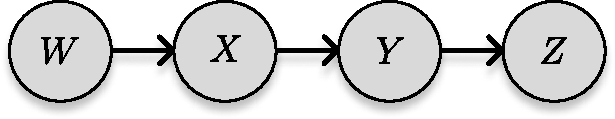
\includegraphics[scale=.29]{figures/chain4.pdf} 
        \caption{chain4} 
    \end{subfigure} 
    \begin{subfigure}[t]{.29\linewidth}
        \centering 
        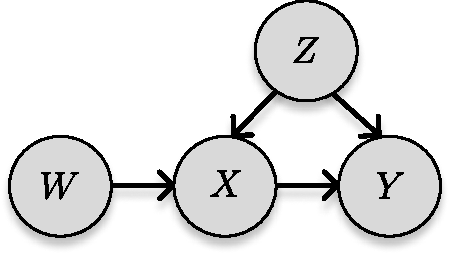
\includegraphics[scale=.29]{figures/iv.pdf} 
        \caption{IV} 
    \end{subfigure}
    \begin{subfigure}[t]{.29\linewidth} 
        \centering 
        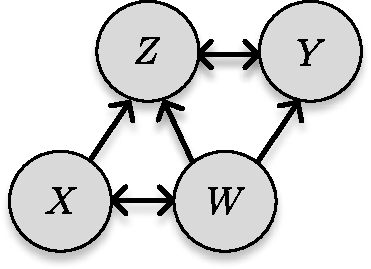
\includegraphics[scale=.29]{figures/collfork.pdf} 
        \caption{collfork}  
    \end{subfigure}
    \caption{\textbf{Ancestral graphs} representing the data generating models for the three considered datasets in Table~\ref{tab:table}.} 
    \label{fig:datasets}
\end{figure} 

\noindent\textbf{Data.} We generate $10$ datasets with $500$ independent samples from the randomly parametrized linear Gaussian SCMs corresponding to the canonical causal diagram \cite{richardson2002ancestral} in each AG depicted in Figure~\ref{fig:datasets}. 
% In a canonical causal diagram, all directed edges in the AG are included, and for each bidirected edge $V_i \leftrightarrow V_j$, a latent variable $U_{ij}$ is introduced as a shared cause for $V_i$ and $V_j$. 
Unshielded colliders and discriminating paths are fundamental patterns in the detection of invariances by CD algorithms under latent confounding \cite{spirtes1997equiv, zhang2008fci}. Thus, we consider the following 4-node causal diagrams with increasingly difficult configurations: (i) \texttt{chain4}, a chain without latent confounders; (ii) \texttt{collfork}, a graph with triplets involving colliders and non-colliders under latent confounding, and (iii) \texttt{IV}, a structure with a discriminating path for $Z$: $W \rightarrow X \leftarrow Z \rightarrow Y$. 

\vspace{0.1pt}

% we computed the PAG corresponding to each of the AGFN's samples by using the d-separation criterion induced by graph as a conditional indepedence oracle.  

% used the d-separation induced by each of the AGFN's samples as conditional independences oracles in FCI to  

% For fairness, we generated $100$ bootstrapped versions of each dataset to estimate the probability distribution induced by the deterministic algorithms (i), (ii) and (iii). The goal is to properly extract probabilitistic features from these deterministic methods. 

% The reported values are averages. 

% The standard deviation of the most rewarding samples is not comparable to the other reported standard deviations. 

% To implement them, we followed the instructions available at these algorithms' public repositories. 



\noindent\textbf{Baselines.} We compare AGFN with four notable CD methods: 
FCI \citep{spirtes2001causation, zhang2008fci}, GFCI \citep{ogarrio2016gfci}, DCD \citep{bhattacharya2021differentiable}, and N-ADMG \cite{ashman2023causal}.
% Fast Causal Inference (FCI), Greedy FCI (GFCI), Differentiable Causal Discovery (DCD), and Neural ADMG Learning (N-ADMG) \citep{zhang2008fci, ogarrio2016gfci, bhattacharya2021differentiable, ashman2023causal}. 
The baselines span four broad classes of CD methods. FCI is a seminal constraint-based CD algorithm that learns a PAG consistent with conditional independencies entailed by statistical tests. GFCI is a hybrid CD algorithm that learns a PAG by first obtaining an approximate structure using FGS \citep{ramsey2015scaling} (a BIC-score-based search algorithm %designed 
for causally sufficient scenarios) and then by applying FCI %orientation rules 
to identify possible confounding and remove some edges added by FGS. DCD casts CD as continuous optimization with differentiable algebraic constraints defining the space of AGs and uses gradient-based algorithms to solve it. N-ADMG computes a variational approximation of the joint posterior distribution over the space of bow-free causal diagrams \citep{nowzohour2017distributional} associated with non-linear SCMs with additive noise. While N-ADMG focuses on a more restricted setting compared to AGs, it offers some uncertainty quantification in the variational pohttps://www.overleaf.com/project/650454a084b798332af29ebesterior, making it more closely comparable to our approach. We rigorously follow the experimental guidelines in the original works.
\vspace{0.1pt}

\noindent\textbf{Experimental setup} We train AGFN on each dataset and use it to sample 100k graphs. 
We also apply FCI, GFCI, and DCD to $100$ bootstrapped resamplings of each dataset to emulate \emph{confidence} distributions induced by these algorithms. 
%
%We used these samples to compute both the mean and standard deviation of the BIC and the SHD.  %w.r.t. the underlying causal diagram. 
%\
To compare the algorithms' outputs, we compute the sample mean and standard deviation of the BIC and SHD at the PAG level. 
%
Specifically, we compute the SHD between the ground-truth PAG and each estimated PAG obtained by each method. 
%
If the output is a PAG member (as for DCD, N-ADMG, and AGFN) we use FCI to transform the output using these graphs as oracles for conditional independencies.
%
Furthermore, we directly compute the BIC for the outputs, as all PAG members are asymptotically score-equivalent.



\noindent\textbf{Results.} \Cref{tab:table} compares AGFN against baseline CD algorithms. Notably, our method consistently outperforms the only probabilistic baseline in the literature (N-ADMG) in terms of both SHD and BIC. As expected, however, the average BIC and SHD induced by AGFN are larger than those induced by the bootstrapped versions of the non-probabilistic algorithms, and the variances are greater; this is due to the inherent sampling diversity of our method and the resulting generation of possibly implausible samples. Indeed, Table~\ref{tab:tablee} shows that the three most rewarding samples from AGFN are as good as (and sometimes better than) the other CD algorithms. Results for N-ADMG comprise the three most frequent samples from the variational distribution. 


\begin{table}
    \centering
    \resizebox{0.6\linewidth}{!}{
    \begin{tabular}{c|c|c|c}
        & chain4 & IV & collfork \\ 
        \hline 
         FCI & $2.07 \textcolor{gray}{ { \scriptstyle \pm 2.00 }}$ & $3.83 \textcolor{gray}{ { \scriptstyle \pm 2.90 }}$ &  $5.43 \textcolor{gray}{ { \scriptstyle \pm 1.87 }}$ \\
         GFCI & $\mathbf{1.50} \textcolor{gray}{ { \scriptstyle \pm 1.63 }}$ & $3.63 \textcolor{gray}{ { \scriptstyle \pm 3.16 }}$ &  $5.53 \textcolor{gray}{ { \scriptstyle \pm 2.11 }}$ \\ 
         DCD & $2.27 \textcolor{gray}{ { \scriptstyle \pm 1.46 }}$ & $4.80 \textcolor{gray}{ { \scriptstyle \pm 2.17 }}$ & $5.60 \textcolor{gray}{ { \pm \scriptstyle 2.13 }}$\\ 
         N-ADMG (top 3) & $4.38 \textcolor{gray}{ {\scriptstyle \pm 0.81} }$ & $6.08 \textcolor{gray}{ {\scriptstyle \pm 1.77} }$ & $6.87 \textcolor{gray}{ {\scriptstyle \pm 0.93} }$ \\ 
         AGFN (top 3) & $2.00 \textcolor{gray}{ {\scriptstyle \pm 1.55 } }$ & $\mathbf{3.50} \textcolor{gray}{ {\scriptstyle \pm 3.29 } }$ &  $\mathbf{4.90} \textcolor{gray}{ {\scriptstyle \pm 2.70 } }$
    \end{tabular}
    }
    \caption{\textbf{SHD for point estimates.} The mean SHD of the top-3 AGFN draws is comparable to or better than baselines.  
    %\vspace{-2pt}
    }
    \label{tab:tablee}
\end{table}


\begin{figure*}[!t] 
    \centering
    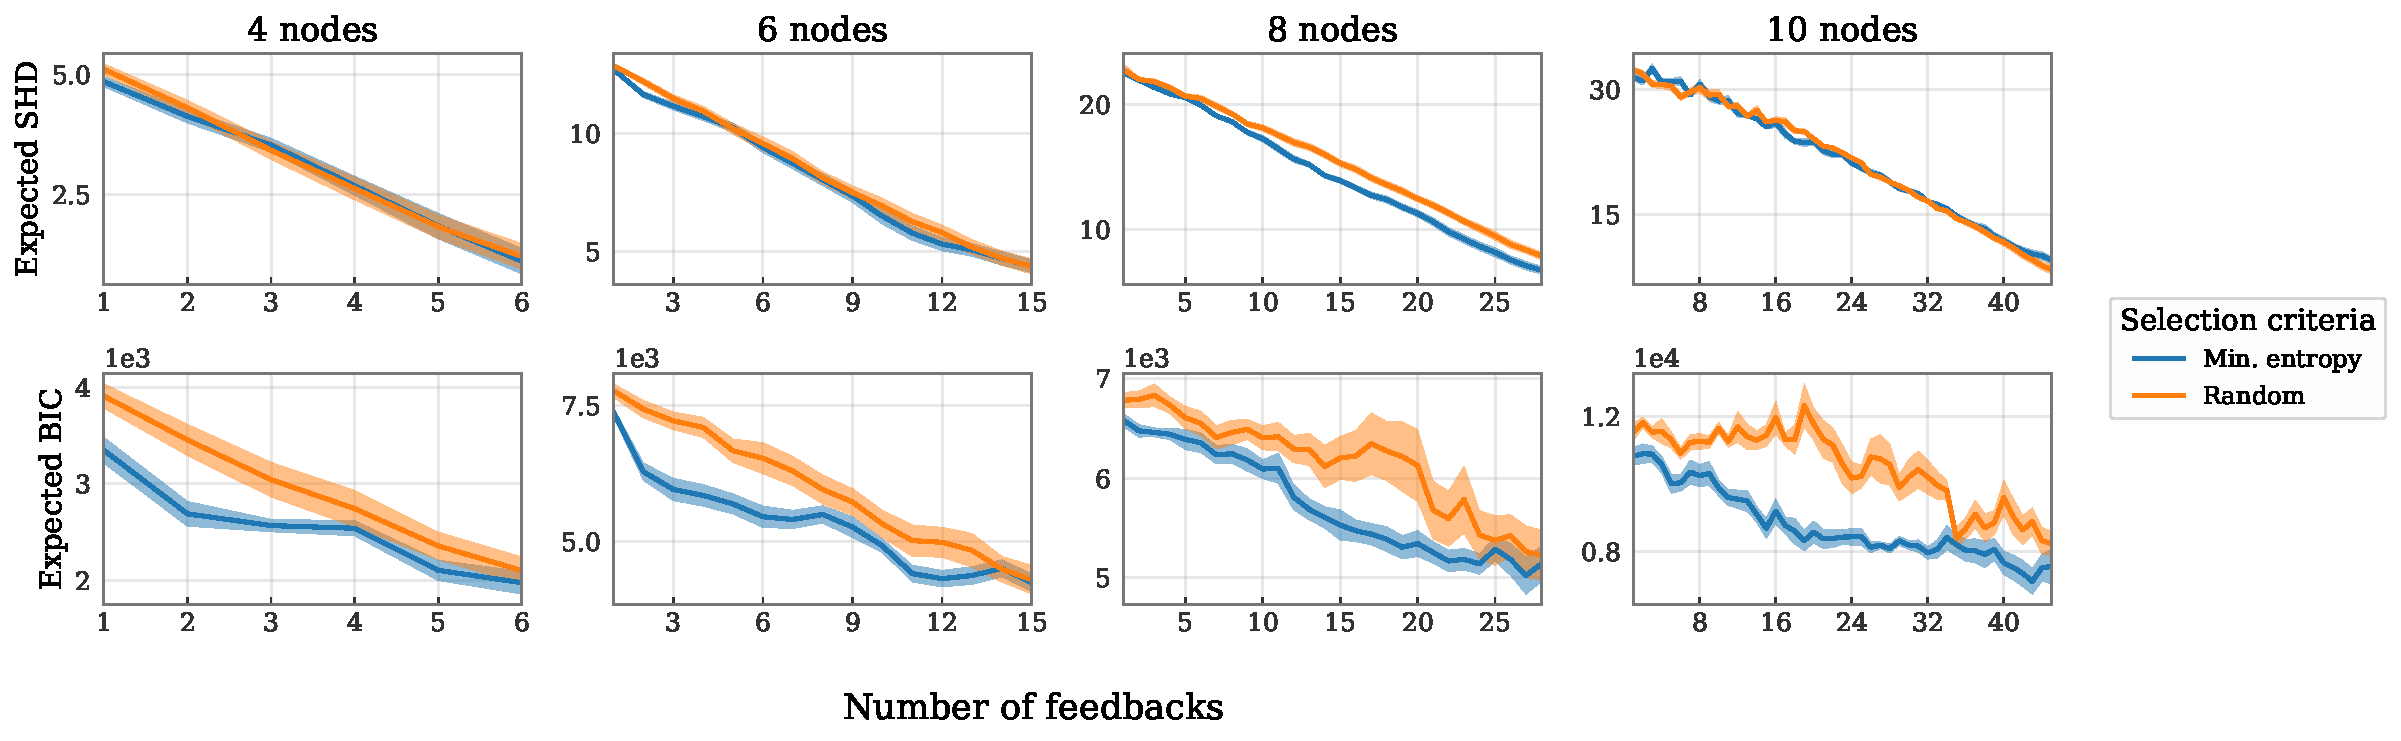
\includegraphics[width=\textwidth]{figures/hitl2.pdf} 
    \caption{\textbf{CD with simulated human feedback.} The top/bottom row shows the mean SHD/BIC of AGFN samples as a function of human interactions. Probing the expert about the edge that minimizes the mean cross-entropy leads to a faster decrease in BIC compared to a random strategy. The SHD decreases similarly in both cases. Results reflect the outcomes of 30 simulations.}
    \label{fig:feedbacks}
\end{figure*}

\subsection{Simulating humans in the loop} 

\noindent\textbf{Data.} We follow the procedure from \Cref{sec:a} to generate graphs with $4$, $6$, $8$ and $10$ nodes. We draw $500$ samples from a compatible linear Gaussian SCM and use them to train an AGFN. Then, we follow our active elicitation strategy from \Cref{sec:hitl} to probe simulated humans, adhering to the generative model described in the same section, with $\pi = 0.9$.


\noindent\textbf{Setup.} Since we are the first to propose an optimal design for expert knowledge elicitation, there are no baselines to compare AGFN against. That being said, we aim to determine whether the inclusion of expert feedback enhances the concentration of the learned distribution around the true AG, and evaluate the effectiveness of our elicitation strategy. To do so, we measure SHD to the true AG and BIC as a function of the number of expert interactions. 



\noindent\textbf{Results.} Figure~\ref{fig:feedbacks} shows that incorporating expert feedback substantially decreases the expected SHD and BIC under our belief over AGs. On the one hand, the remarkable decrease in expected SHD shows that our belief becomes increasingly focused on the true AG as we iteratively request the expert's feedback, regardless of the querying strategy. On the other hand, the second row shows that our querying strategy results in a substantial decrease in the BIC, demonstrating a faster reduction than random queries. This validates the notion that some edges are more informative than others, and we should prioritize them when probing the expert. 

\section{Related Work}

\noindent \textbf{CD under latent confounding.}
Following the seminal works by \citet{spirtes2001causation} and \citet{zhang2008fci} introducing the complete FCI, a variety of works have emerged. Among them are algorithms designed for sparse scenarios, including RFCI \citep{colombo2012rfci} and others \citep{silva2013mcmc, claassenMH13}. Notably,  \citet{silva2013mcmc}'s framework uses a Bayesian approach to CD of Gaussian causal diagrams based on sparse covariance matrices. Nonetheless, it requires sampling one edge at a time and relies on numerical heuristics that might effectively alter the posterior we are sampling from. \citet{colombo2012rfci} introduced the conservative FCI to handle conflicts arising from statistical errors in scenarios with limited data, even though it yields less informative results. Subsequent efforts to improve reliability led to the emergence of constraint-based CD algorithms based in Boolean satisfiability \citep{hyttinen2014constraint, magliacane2016ancestral}, although they are known to scale poorly on $|\mathbf{V}|$ \citep{lu2021improving}. In another paradigm, score-based search algorithms rank MAGs according to goodness-of-fit measures, commonly using BIC for linear Gaussian SCMs 
\citep{triantafillou2016score, zhalama2017sat, DBLP:conf/uai/RantanenHJ21}. There are also hybrid approaches that combine constraint-based strategies to reduce the search space, such as GFCI~\citep{ogarrio2016gfci}, M3HC~\citep{tsirlis2018m3hc}, BCCD~\citep{classen2012bccd}, and GSPo~\citep{bernstein2020ordering}. 
Continuous optimization approaches have recently emerged as a novel approach to score-based CD, such as DCD \citep{bhattacharya2021differentiable} and N-ADMG \cite{ashman2023causal}.


\noindent\textbf{CD with expert knowledge.}  Previous works on CD have explored various forms of background knowledge. This includes knowledge on edge existence/non-existence \cite{DBLP:conf/uai/Meek95a}, ancestral constraints \cite{DBLP:conf/nips/ChenSCD16}, variable grouping \cite{DBLP:journals/ijar/ParviainenK17}, partial order \cite{DBLP:conf/aistats/Andrews20} and typing of variables \citep{DBLP:conf/clear2/BrouillardTLLD22}. Incorporating expert knowledge is pivotal to reducing the search space and the size of the learned equivalence class. However, due to significant challenges, up to date, there are only a few works trying to integrate human knowledge into CD within the context of latent confounding~\citep{DBLP:conf/aistats/Andrews20, DBLP:conf/nips/WangQZ22}. These works operate under the assumption of perfect expert feedback. In contrast, our contribution is novel in that it confronts the challenges of real-world situations where expert input might be inaccurate. 
% Exploring the integration of features from both methods holds the potential for promising avenues in future research.

% Existing works include 
% \cite{DBLP:conf/aistats/Andrews20}, which enables the incorporation of a hierarchical arrangement of nodes in the FCI, and 
% \cite{DBLP:conf/nips/WangQZ22}. %\cite{DBLP:journals/ai/WangQZ23, DBLP:conf/nips/WangQZ22}
%Recent advancements in CD with latent variables have 
%\cite{DBLP:journals/ai/WangQZ23, DBLP:conf/nips/WangQZ22}
% which proposes orientation rules that incorporate local background knowledge, complemented by an active learning algorithm for iterative refinement. However, the validity of this method relies on the accuracy of the initial MEC and the knowledge contributed by experts, which includes information on the edge marks. 


% \vspace{2pt}



% \noindent\textbf{GFlowNets for inference in graphical models.} 
% To address uncertainty modeling of the graph structure, recent advances in \emph{Generative Flow Networks} \citep[GFlowNets;][]{bengio2021GFlowNet,bengio2021GFlowNetfoundations, deleu2022bayesian} have shown promise in approximating a posterior distribution over 
% Bayesian networks (BNs), which encode conditional independencies using
% directed acyclic graphs (DAGs).
% Formally, let $\mathcal{G}$ represent a space of DAGs over $\mathcal{X}$. The goal is to approximate the posterior distribution $p(\mathcal{G}|\mathcal{D})$ that captures the uncertainty in the DAG structure given the observational data. % Under the assumption of causal sufficiency, BNs represent causal DAGs, 



\section{Discussion}

We presented AGFN, the first probabilistic CD method that accounts for latent confounding and incorporates potentially noisy human feedback in the loop. AGFN samples AGs according to a score function, quantifying the uncertainty in the learning process. Furthermore, it can leverage human feedback in an optimal design strategy, efficiently reducing our uncertainty on the true data-generating model. 

This work is focused on linear Gaussian models, using BIC as our score. However, the implementation of AGFNs is not restricted by this choice. In principle, we could replace the BIC with alternative score functions that are more appropriate for different types of variables, e.g. for discrete data \citep{drton2008binary}.
%
It is also important to highlight that our framework does not require retraining the AGFN after we see human feedback. Moreover, AGFN is a GPU-powered algorithm, and while we used only one GPU in our experiments, it is possible to greatly accelerate AGFN by using cluster architectures with multiple GPUs.


By offering uncertainty-quantified CD together with a recipe for including humans in the loop, 
we expect AGFNs will significantly enhance the accuracy and reliability of CD, especially in real-world domains. 
Moreover, AGFNs bring a novel perspective to developing more comprehensive tools for downstream causal tasks \cite{bareinboim2016pnas}, as the resulting distribution encodes knowledge from data and human feedback while accounting for epistemic uncertainty. For example, methods for causal reasoning that currently rely on a single AG \cite{DBLP:journals/jmlr/Zhang08, jaber2022pagid} could exploit this distribution to incorporate a richer understanding of uncertainty and knowledge, thereby enhancing their robustness and reliability. 


\section*{Acknowledgments}
Diego Mesquita acknowledges the support by the Fundação Carlos Chagas Filho de Amparo à Pesquisa do Estado do Rio de Janeiro FAPERJ (SEI-260003/000709/2023), the São Paulo Research Foundation FAPESP (2023/00815-6), the Conselho Nacional de Desenvolvimento Científico e Tecnológico CNPq (404336/2023-0), and the Silicon Valley Community Foundation through the University Blockchain Research Initiative (Grant \#2022-199610).
%
António Góis acknowledges the support by Samsung Electronics Co., Ldt. 
%
Adèle Ribeiro and Dominik Heider were supported by the LOEWE program of the State of Hesse (Germany) in the Diffusible Signals research cluster and by the German Federal Ministry of Education and Research (BMBF) [031L0267A] (Deep Insight).
%
Samuel Kaski was supported by the Academy of Finland (Flagship programme: Finnish Center for Artificial Intelligence FCAI), EU Horizon 2020 (European Network of AI Excellence Centres ELISE, grant agreement 951847), UKRI Turing AI World-Leading Researcher Fellowship (EP/W002973/1).
%
We also acknowledge the computational resources provided by the Aalto Science-IT Project from Computer Science IT.


\newpage 

\appendix 

%%% nao pode usar 
\clearpage
\appendix

\section{Additional Related Works} 
% \noindent \textbf{Additional Related Works}

\noindent \textbf{Generative Flow Networks} \citep[GFlowNets;][]{bengio2021GFlowNet, bengio2021GFlowNetfoundations} are generative models that sample discrete composite objects from an unnormalized reward function.
%GFlowNets diverse modes while avoiding the mixing time of MCMC methods.
They have been successfully used to sample various structures such as protein sequences~\citep{dna} and schedules~\citep{zhang2023robust}. They have also been used to train energy-based models \citep{zhang2022energy}. In the field of structure learning, they have been applied to Bayesian networks --- more specifically to sample a posterior over DAGs in linear Gaussian networks, although without accounting for unobserved confounding \citep{deleu2022bayesian}. Recently, \citet{deleu2023joint} proposed an extension to jointly infer the structure and parameters, also grounded in the assumption of causal sufficiency. It is worth highlighting that training GFlowNets in these scenarios presents optimization challenges, resulting in the utilization of a variety of loss functions \citep{shen2023towards}. Moreover, \citet{lahlou2023continuous} proposed an extension of GFlowNets to continuous domains. 

% \textcolor{red}{I guess here we just want to list a bunch of Gflownet references. The first 6 lines can be severely summarized :) Then, the torrent of references.}


%GFlowNets are deep generative models for graphs and have been successfully used to sample various structures such as Bayesian networks~\citep{deleu2022bayesian}, schedules~\citep{zhang2023robust}, and protein sequences~\citep{dna}. 

% The FCI algorithm \citep{spirtes2001causation}
% combined with \citep{zhang2008fci}'s complete set of orientation rules is the first asymptotically sound and complete constraint-based algorithm for scenarios under latent confounding. In real-world scenarios, the reliability of FCI heavily relies on the oracle of conditional independence relations. %MEC of MAGs, %Maximal Ancestral Graphs (MAGs), 
% %referred to as \textit{Partial Ancestral Graph (PAG)}. 
% To tackle the lack of robustness of the FCI in limited data regimes, \citep{colombo2012learning} proposed the Conservative FCI (CFCI). The CFCI performs additional conditional independence tests to identify unfaithful triplets before the orientation phase, which then exclusively relies on unambiguous triples. Nevertheless, the resulting output is typically less informative. Also as an effort to enhance robustness and resolve conflicting constraints arising from statistical errors, a novel class of constraint-based CD algorithms has emerged \cite{hyttinen2014constraint, magliacane2016ancestral}. These algorithms map data-derived conditional independencies into logical constraints regarding (non-)ancestral relationships and then learn a MEC of Ancestral Graphs through Boolean satisfiability (SAT) solvers. However, their accuracy still depends on the reliability of the oracle of conditional independencies and currently, they have significant limitations in terms of scalability \citep{lu2021improving}. %(It works very well on small-scale problems (less than 8 variables). https://ojs.aaai.org/index.php/AAAI/article/view/17059
% % by employing Boolean satisfiability solvers
% % which defines a class of causal structures (that can be found 
% %[Triantafilou et al., 2010, Hyttinen et al., 2013, 2014, Triantafillou and Tsamardinos, 2015, Borboudakis and Tsamardinos, 2016, Magliacane et al., 2016]

%  %Bayesian Information Criterion (BIC). 
% Similar to our work, the vast majority of score-based CD algorithms for settings with latent confounding assume the causal model is a linear Gaussian SCM and then rely on the BIC score. The first proposed is GSMAG %Greedy Search for MAGs (GSMAG)
% by \citep{triantafillou2016score}, which employs a simple greedy hill-climbing procedure to explore the space of all potential MAGs, aiming to find the structure that optimizes the BIC. The optimal MAG functions as a surrogate for identifying the PAG corresponding to the true underlying causal model.  
% Building upon the GSMAG, several hybrid approaches, such as GFCI, M3HC, and GSPo % Greedy Sparsest Poset  %(MMHC for MAGs), 
% have been proposed \cite{ogarrio2016gfci, tsirlis2028m3hc, bernstein2020ordering}. These approaches combine constraint-based strategies to reduce the space of structures to investigate. In particular, the GFCI first uses the FGS %Fast Greedy Search (FGS) 
% algorithm \cite{ramsey2015scaling} to identify an approximated structure and then applies the FCI orientation rules to both identify possible confounding and remove some of the edges added by FGS. The GSPo algorithm leverages the mapping of MAGs to partially ordered sets (posets), effectively reframing the CD  problem as the task of learning a poset.
% %These search-based algorithms are 
% Acknowledging the lack of guarantees on the optimality of the learned MAG from greedy and hybrid greedy algorithms, \citep{DBLP:conf/uai/RantanenHJ21} propose the MAGSL. This method employs dynamic programming and branch-and-bound techniques to learn a globally optimal MAG. Despite conducting an exact search, the algorithm's effectiveness relies on specific sparsity conditions, delineated by constraints on both the size of the c-components and the maximum number of parents that a c-component can possess.

% Recently, continuous optimization approaches have emerged as a novel category of CD algorithms. Utilizing an approximate BIC score, \citep{bhattacharya2021differentiable} introduce Differentiable Causal Discovery (DCD). Initially, they establish differentiable algebraic constraints that define the space of AGs. Then, they formulate the CD task as a continuous optimization problem and design differentiable procedures to find the best-fitting ADMG. More recently, \cite{ashman2023causal} propose N-ADMG %Neural ADMG Learning (N-ADMG), 
% which is based on neural causal models and extends diffD to scenarios where the underlying causal diagram is bow-free and corresponds to a non-linear SCM with additive noise. It employs variational inference to approximate the posterior distribution over causal diagrams and learns the model parameters via gradient-based optimization. While N-ADMG focuses on a more restricted setting compared to that of AGs, it facilitates uncertainty quantification through the sampling of causal diagrams from the learned posterior, rendering it more closely comparable to our approach.


% \section{Additional details on AGFN}

\section{Cross-entropy acquisition}

The expected \textit{mutual information} and the \textit{information gain} are the most widely used information-theoretic measures to actively interact with a human and choose the most informative data points to be labeled \cite{ryan15bayesian}. However, we instead use the negative expected cross-entropy between the current and updated beliefs as the acquisition function of our experimental design (see \cref{eq:divergence}). As we show next, the approximation of both the mutual information and the information gain is intrinsically dependent upon the estimation of the log-partition of the updated beliefs over the space of ancestral graphs. Doing so is computationally intensive, and we would either need to use a Monte Carlo estimator of the integrals or use some posterior approximation --- in both cases, leading to asymptotically biased estimates of the acquisition. In contrast, we can easily leverage AGFN samples to compute asymptotically unbiased estimates of our acquisition function.  The next paragraphs provide further details.

\paragraph{Mutual information.} The \textit{mutual information} between two random variables $X$ and $Y$ with joint distribution $p(X, Y)$ and marginal distributions $p(X)$ and $p(Y)$ is  
\begin{equation}
    I(X, Y) = \mathcal{D}_{KL}[ p(X, Y) || p(X) \otimes p(Y)], 
\end{equation}
in which $\mathcal{D}_{KL}$ is the Kullback-Leibler divergence. In this context, an alternative approach to our experimental design for active knowledge elicitation would consist in iteratively maximizing the expected mutual information between the observed samples, $\mathcal{G}$, and the elicited feedback, $f_{K}$, to select the relation about which the expert would provide feedback. More specifically, we could choose 
\begin{equation} \label{eq:mutualinformation}  
    r_{K + 1} = \argmax_{r \in {\mathbf{V} \choose 2}} \mathbb{E}_{f_{r} \sim p(\cdot | \mathbf{f}_{K})} [ I(\mathcal{G}, f_{r}) ], 
\end{equation}
in which 
\begin{equation} 
    I(\mathcal{G}, f_{r}) = \mathcal{D}_{KL}[ q(\mathcal{G}, f_{r} | \mathbf{f}_{K}) || q(\mathcal{G} | \mathbf{f}_{K}) \otimes p(f_{r} | \mathbf{f}_{K})], \label{eq:MI}
\end{equation}
at each interaction with the expert. Nonetheless, note that  
\begin{align*}
    &q(\mathcal{G}, f_{r} | \mathbf{f}_{K}) = q(\mathcal{G} | \mathbf{f}_{K + 1}) p(f_{r} | \mathbf{f}_{K}) \\ & = c_{K + 1}(f_{r}) p_{\theta}(\mathcal{G}) \left(\prod_{1 \le k \le K + 1} p(\omega_{r_{k}} | f_{r_{k}})\right) \cdot p(f_{r} | \mathbf{f}_{K}),  
\end{align*} 
with $f_{r_{K + 1}} = f_{r}$ and 
\begin{equation} \label{eq:partition} 
    c_{K + 1}(f_{r}) = \left(\!\!\sum_{\mathcal{G}} p_{\theta}(\mathcal{G}) \!\! \left(\prod_{1 \le k \le K + 1} p(\omega_{r_{k}} | f_{r_{k}}) \!\!\right)\!\!\right)^{-1} 
\end{equation}
as the partition function of our updated beliefs. Note also that \Cref{eq:MI} entails computing the entropy of  $q(\mathcal{G}, f_r | \mathbf{f}_K)$. Thus, the selection criterion in \cref{eq:mutualinformation} requires an accurate estimate of $\log c_{K + 1}(f_{r})$ --- which is well-known for being a difficult problem \cite{ma13partition} --- and the Monte Carlo estimator for the log-partition function is asymptotically biased. % Hence, we do not use the mutual information between the observed samples and the pursued feedback as a criterion for our active knowledge elicitation.  

% \begin{equation}
%     c(f_{r}) = \sum_{G} p_{\theta}(\mathcal{G}) \left(\prod_{1 \le k \le K + 1} p(f_{r_{k}} | \omega_{r_{k}}) \right), 
% \end{equation}

% the selection criterion in Equation

\paragraph{Information gain.} The expected \textit{information gain} of an elicitation is defined as the expected KL divergence between our updated and current beliefs over ancestral graphs. This approach is widely employed in Bayesian experimental design \cite{ryan15bayesian}. In our framework, the information gain resulting from a feedback $f_{r}$ is 
\begin{equation} % \label{eq:informationgain}  
    \text{IG}_{K}(f_{r}) = \mathcal{D}_{KL}[ q(\mathcal{G} | \mathbf{f}_{K} \cup f_{r}) || q(\mathcal{G} | \mathbf{f}_{K})],  % . 
\end{equation}
which yields the criterion 
\begin{equation} \label{eq:informationgain} 
    r_{K + 1} = \argmax_{r \in {\mathbf{V} \choose 2}} \mathbb{E}_{f_{r} \sim p(\cdot | \mathbf{f}_{K})} \left[ \text{IG}_{K}(f_{r}) \right].   
\end{equation}
Nonetheless, \cref{eq:informationgain} suffers from the same problems of \cref{eq:mutualinformation}: it requires approximating the logarithm of the partition function $c_{K + 1}(f_{r})$ of a distribution over the combinatorially large space of ancestral graphs, which is notably very challenging to estimate. Indeed, as 
\begin{align*}
    \mathcal{D}_{KL} [ q(\mathcal{G} | \mathbf{f}_{K + 1}) || q(\mathcal{G} | \mathbf{f}_{K}) ] = \underset{\mathcal{G} \sim q(\cdot | \mathbf{f}_{K + 1}) }{\mathbb{E}} \left[ \log \frac{q(\mathcal{G} | \mathbf{f}_{K + 1})}{q(\mathcal{G} | \mathbf{f}_{K})} \right] \\ 
    = \underset{\mathcal{G} \sim q(\cdot | \mathbf{f}_{K + 1})}{\mathbb{E}} \left[ \log p(f_{r} | \omega_{r}) + \log c_{K + 1}(f_{r}) - \log c_{K} \right], 
\end{align*}
with $f_{r_{K + 1}} = f_{r}$, $c_{K}$ as the partition function of $q(\cdot | \mathbf{f}_{K})$ --- that does not depend upon $f_{r}$ ---, and $c_{K + 1}(f_{r})$ defined in \cref{eq:partition}, the estimation of the information gain is inherently dependent upon the estimation of the log-partition function. % Thus, we disregard this alternative as a selection criterion of our framework for active knowledge elicitation due to its statistical difficulty and computational intractability. 

% Thus, we disregard this alternative as an selection criterion for our framework for active knowledge elicitation. 

\paragraph{Cross-entropy.} The cross-entropy between our updated and current beliefs is an intuitively plausible and practically useful strategy to interact with an expert efficiently. In fact, since 
\begin{equation*}
\begin{split}
    \mathbf{H}&[q(\cdot | \mathbf{f}_{K + 1}), q(\cdot | \mathbf{f}_{K})]\\ 
    &= \underset{\mathcal{G} \sim q(\cdot | \mathbf{f}_{K + 1})}{\mathbb{E}} [- \log q(\mathcal{G} | \mathbf{f}_{K})] \\ 
    &= \underset{\mathcal{G} \sim q(\cdot | \mathbf{f}_{K + 1})}{\mathbb{E}} \left[ - \log p_{\theta}(\mathcal{G}) - \sum_{1 \le k \le K} \log p(\omega_{r_{k}} | f_{r_{k}}) - l_{K} \right]
\end{split}, 
\end{equation*}
\noindent in which $l_{K}$ is the log-partition function of the distribution $q(\cdot | \mathbf{f}_{K})$. Further, the cross-entropy depends exclusively upon i) the logarithm of the samples' rewards, $\log p_{\theta}(\mathcal{G})$, which is readily computed within AGFN's generative process, and ii) the posterior distribution over the relations' features $\omega_{r}$ given the expert's feedbacks $f_{r}$, which is available in closed form. Hence, the previously mentioned expectation is unbiasedly and consistently estimated by our importance sampling scheme. Furthermore, our empirical findings in \cref{fig:feedbacks} suggest that the cross-entropy yields good results and consistently outperforms a uniformly random strategy with respect to the BIC score. 

% \begin{equation}
%     \mathcal{D}_{KL}[ q(\mathcal{G} | \mathbf{f}_{K + 1}) || q(\mathcal{G} | \mathbf{f}_{K}) ] = \mathbb{E}_{G \sim q(\cdot | \mathbf{f}_{K + 1})} [ \log \frac{q(\mathcal{G} | \mathbf{f}_{K + 1})}{q(\mathcal{G} | \mathbf{f}_{K})}] 
% \end{equation}


\section{Experimental details} 

We lay out the experimental and implementational details of our empirical analysis in the next subsections. In \Cref{sec::baselines}, we describe the specific configurations of the CD algorithms that we compared with our method in \cref{tab:tablee}. Then, we consider in \cref{sec::training} some practical guidelines and architectural specifications that enable us to train and make inferences with AGFN efficiently. Finally, we contemplate in \cref{sec::hitl} the algorithmic details for simulating the expert's feedback according to our model for active knowledge elicitation. 

% Then, we consider in \cref{sec::training} some practical guidelines and architectural specifications that enable us to efficiently train and make inferences with AGFN. 

% We provide further empirical details in this section. Specifically, we include in \cref{sec::training} an ablation study for the parametrizations we proposed for AGFN's flows and some practical guidelines regarding the implementation of our method. Then, we lay out in \cref{sec::hitl} the algorithmic details of our Bayesian scheme for modeling the epistemic uncertainty within the expert's knowledge.   

% Then, we lay out in \cref{sec::hitl} the algorithimc details 

\subsection{Baselines} \label{sec::baselines} 

\paragraph{FCI.} For the results in \cref{tab:table}, we first estimated a PAG using the stable version of FCI, which produces a fully order-independent final skeleton \citep{colombo2014order}. To identify conditional independencies, we used Fisher's Z partial correlation test with a significance level of $\alpha = 0.05$. The BIC score associated with the PAG estimated by the FCI was computed as the BIC of a randomly selected maximal AG (MAG) within the equivalence class characterized by such PAG. The maximality of an AG depends on the absence of inducing paths between non-adjacent variables, which are paths where every node along it (except the endpoints) is a collider and every collider is an ancestor of an endpoint \citep{DBLP:conf/uai/RantanenHJ21}. This ensures that in the MAG every non-adjacent pair of nodes is m-separated by some set of other variables. Importantly, Markov equivalent MAGs exhibit asymptotic equivalence in terms of BIC scores \citep{richardson2002ancestral}. As a result, the choice of a random MAG does not disrupt the validity of our results.  

%In an AG, a path in which every node along it (except the endpoints) is a collider and every collider is an ancestor of an endpoint is termed as an inducing path \citep{DBLP:conf/uai/RantanenHJ21}. If an inducing path exists between two nodes $V_i$ and $V_j$ in an AG $\mathcal{G}$, then there is no set of other variables in $\mathcal{G}$ that can m-separate them. To uphold the pairwise Markov property (where each pair of non-adjacent vertices is m-separated by some set of other variables) in AGs, a common technical requirement is maximality. Formally, a \textit{maximal ancestral graph} (MAG) is defined as an AG with no inducing paths between non-adjacent variables \cite{richardson2002ancestral , DBLP:journals/jmlr/Zhang08}.
%Importantly, MAGs within the same equivalent class are asymptotically distributionally indistinguishable, and thus the selection of a random MAG does not disrupt the validity of our results.    

\paragraph{GFCI.} Similarly, we applied GFCI with an initial search algorithm (FGS) based on the BIC score and the subsequent application of the FCI with conditional independencies identified by the Fisher's Z partial correlation test with a significance level $\alpha = 0.05$. This was performed for all datasets listed in \cref{tab:table}. 
Also similar to the procedure adopted with the FCI,  the BIC score associated with the estimated PAG was computed as the BIC of a randomly selected MAG within the equivalence class characterized by such PAG. 

% We similarly applied GFCI backboned by Fisher-Z's test for conditional independence with a significance level of $\alpha = 0.05$ and a 

\paragraph{DCD.} We adhered to the instructions provided in the official repository\footnote{Available online at \lstinline{https://gitlab.com/rbhatta8/dcd}.} to apply the DCD method on the datasets in \cref{tab:table}. The SHD was obtained between the ground-truth PAG and the PAG corresponding to the estimated ADMG (i.e., the one obtained via FCI by using the d-separations entailed by the estimated ADMG as an oracle for conditional independencies).  
%For the SHD, we used the d-separation induced by DCD's returned ADMG as a conditional independence oracle in FCI to compute the representative PAG; then, we evaluated the SHD between this PAG and the known ground-truth PAG.
On the other hand, the BIC was computed for the estimated ADMG directly. %we used the returned ADMG as the underlying structure for the linear Gaussian SCM and computed the BIC of the ensuing probabilistic model.    

\paragraph{N-ADMG.} To estimate the parameters of the variational distribution defined by N-ADMG, we executed the code provided at the official repository\footnote{Available online at \lstinline{https://github.com/microsoft/causica/releases/tag/v0.0.0}.}  For fairness, we used the same hyperparameters and architectures reported in their original work \cite{DBLP:conf/iclr/LiLSH23}; in particular, we trained the models for $30$k epochs. After this, we sampled $100$k graphs from the learned distribution. It is worth mentioning that the constraints of bow-free ADMG are guaranteed in the N-ADMG samples only in an asymptotic sense. Thus, we manually removed any cyclic graphs from the learned distribution. Then, we proceeded exactly as with DCD to estimate both the average SHD and the average BIC under the variational distribution. %Moreover, we applied the same criterion for validating AGFN's samples (see \cref{sec::training}) and found that over $60$\% of N-ADMG's sampled graphs did not satisfiy the ancestrality constraints of \cref{eq:cond:ancestral}. This is possibly due to the independence between the directed and bidirected edges posited by the variational distribution learned by N-ADMG, which frequently induces almost cycles in the sampled graphs. 

% This is possibly due to the independence between directed and bidirected edges posited by the variational distribution learned by N-ADMG, which frequently induces almost cycles in the sampled graphs. 

\subsection{Implementational details for AGFN} \label{sec::training} 

\begin{figure*}[!t] 
    \centering
    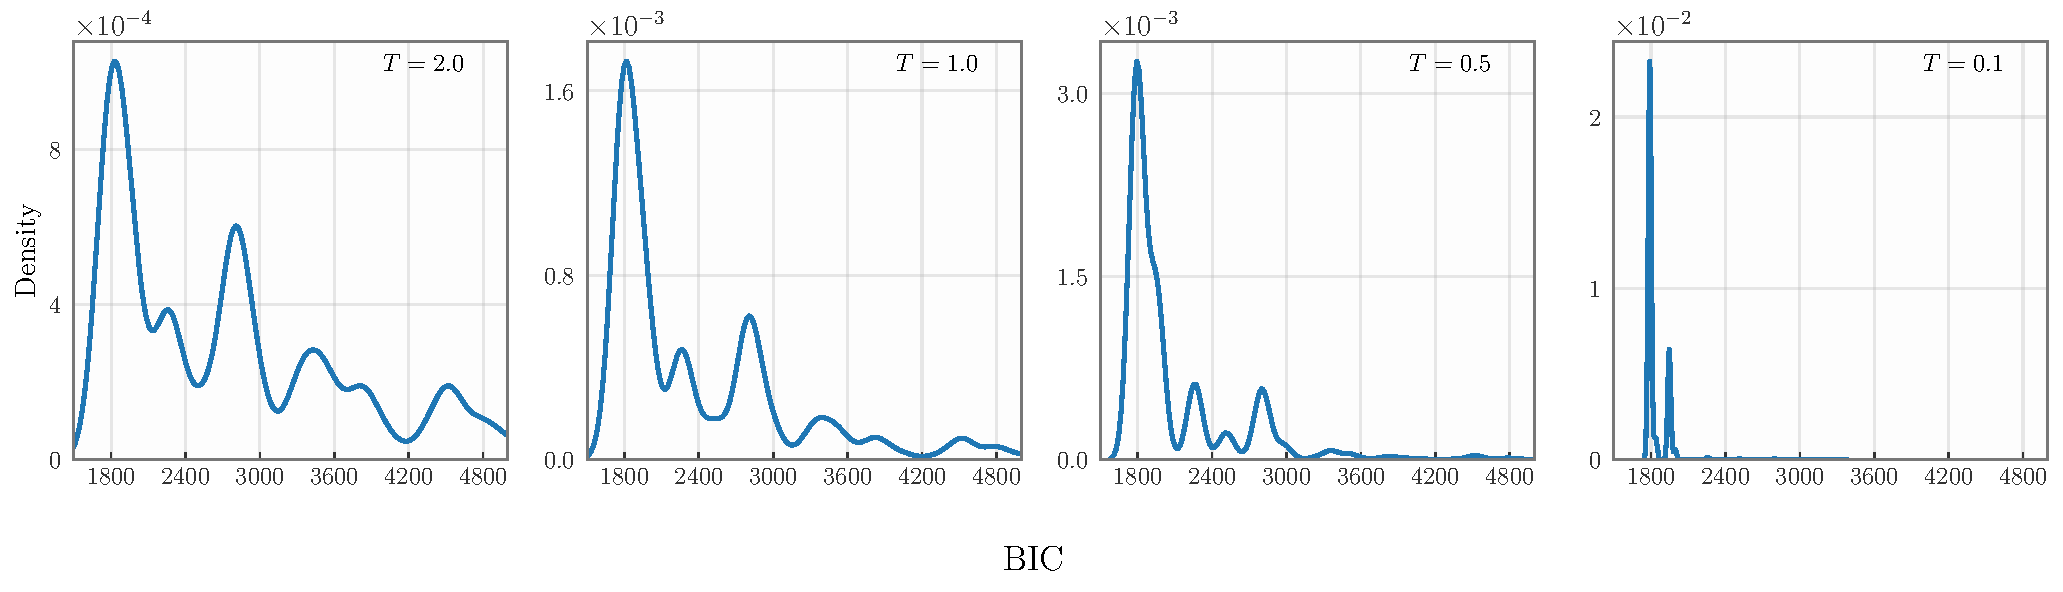
\includegraphics[width=\textwidth]{figures/temperatures.pdf} 
    \caption{\textbf{Tempered rewards}. Training AGFN to sample from increasingly cold distributions (\cref{eq:tempering}) enables us to increase the proportion of high-scoring graphs (i.e., with a low BIC-score) with the drawback of reducing the AGFN's sampling diversity.} 
    \label{fig:tempering}
\end{figure*}

\paragraph{Masking.} To ensure AGFN only samples ancestral graphs, we keep track of a binary mask $\mathbf{m}_{t}$ that indicates which actions lead to a valid state at the iteration $t$ of the generative process; this mask defines the support of the policy evaluated at the corresponding state. In more detail, let $\mathbf{y}_{t}$ be the last layer embedding (prior to a softmax) at iteration $t$ of the neural network used to parametrize the forward flow of AGFN. The probability distribution over the space of feasible actions is then 
\begin{equation*}
    \mathbf{p}_{t} = \text{Softmax} \left( \mathbf{y}_{t} \odot \mathbf{m}_{t} + \epsilon \cdot (1 - \mathbf{m}_{t}) \right) 
\end{equation*}
for a large and negative constant $\epsilon$. We empirically verified that $\epsilon = -10^{5}$ is sufficient to avoid the sampling of non-ancestral graphs. 


\paragraph{Exploratory policy.} During training, we must use an exploratory policy that (i) enables the exploration of yet unvisited states within the pointed DAG and (ii) exploits highly valuable and already visited states. To alleviate this phenomenon, we also draw trajectories from a uniform policy, which is a widespread practice in the literature \citep{bengio2021GFlowNet, deleu2022bayesian, shen2023towards}.  
% More specifically, we employ a convex mixture between a uniform distribution over the states directly reachable from $\mathcal{G}_{t}$ and the currently learned forward policy $\pi_{F}(\cdot | \mathcal{G}_{t})$ \cite{bengio2021GFlowNet, deleu2022bayesian, shen2023towards}. 
More precisely, let $\text{Ch}(\mathcal{G}_{t})$ be the set of states (i.e., ancestral graphs) directly reachable from $\mathcal{G}_{t}$ and $\alpha \in [0, 1]$. At each iteration $t$ of the generative process, we sample an action (either an edge to be appended to the graph or a signal to stop the process)
\begin{equation*}
    a_{t} \sim (1 - \alpha) \cdot \mathcal{U}(\text{Ch}(\mathcal{G}_{t})) + \alpha \cdot \pi_{F}(\cdot | \mathcal{G}_{t}) % .
\end{equation*}
\noindent and modify $\mathcal{G}_{t}$ accordingly. The parameter $\alpha$ quantifies the mean proportion of on-policy actions and represents a trade-off between choosing actions that lead to highly valuable states ($\alpha = 1$) and actions that lead to unvisited states ($\alpha = 0$). We fix $\alpha = \frac{1}{2}$ throughout the experiments. During inference, we set $\alpha = 1$ to sample actions exclusively from the GFlowNet's learned policy. 

% We fix $\alpha = \frac{1}{2}$ throughout the experiments. During inference, we set $\alpha = 1$ to sample actions exclusively from the GFlowNet's learned policy.  

% The parameter $\alpha$ represents a trade-off between exploration and exploitation. 

\paragraph{Detection of invalid states.} We use the algebraic condition in \cref{eq:cond:ancestral} to check whether a graph $\mathcal{G}$ is ancestral. At each iteration of the generative process, we draw an action from the current exploratory policy and test the ancestrality of the updated graph; if it is not ancestral, we revert the sampled action and mask it. Importantly, this protocol guarantees that all graphs sampled from AGFN are ancestral. 

\paragraph{Batch sampling.} We exploit batch sampling to fully leverage the power of GPU-based computing in AGFN. As both the maximum-log-likelihood-based reward and the validation of the states are parallelizable operations, we are able to distribute them across multiple processing units and efficiently draw samples from the learned distribution. Crucially, this end-to-end parallelization substantially improves the computational feasibility of our algorithm and is a notable feature generally unavailable in prior works \cite{zhang2008fci, ogarrio2016gfci, DBLP:conf/uai/RantanenHJ21}. We use a batch size of 256 for all the experiments --- independently of the graph size.  

% We also notice that 
% Noticeably, the use of a graph neural network (GNN) for the forward flow entailed a decrease of 10x in the number of epochs required for successfully training a GFlowNet; this emphasizes the effectiveness of an inductively biased architectural design for the parametrization of GFlowNet's flows. 

\begin{figure*}[!t]
    \centering
    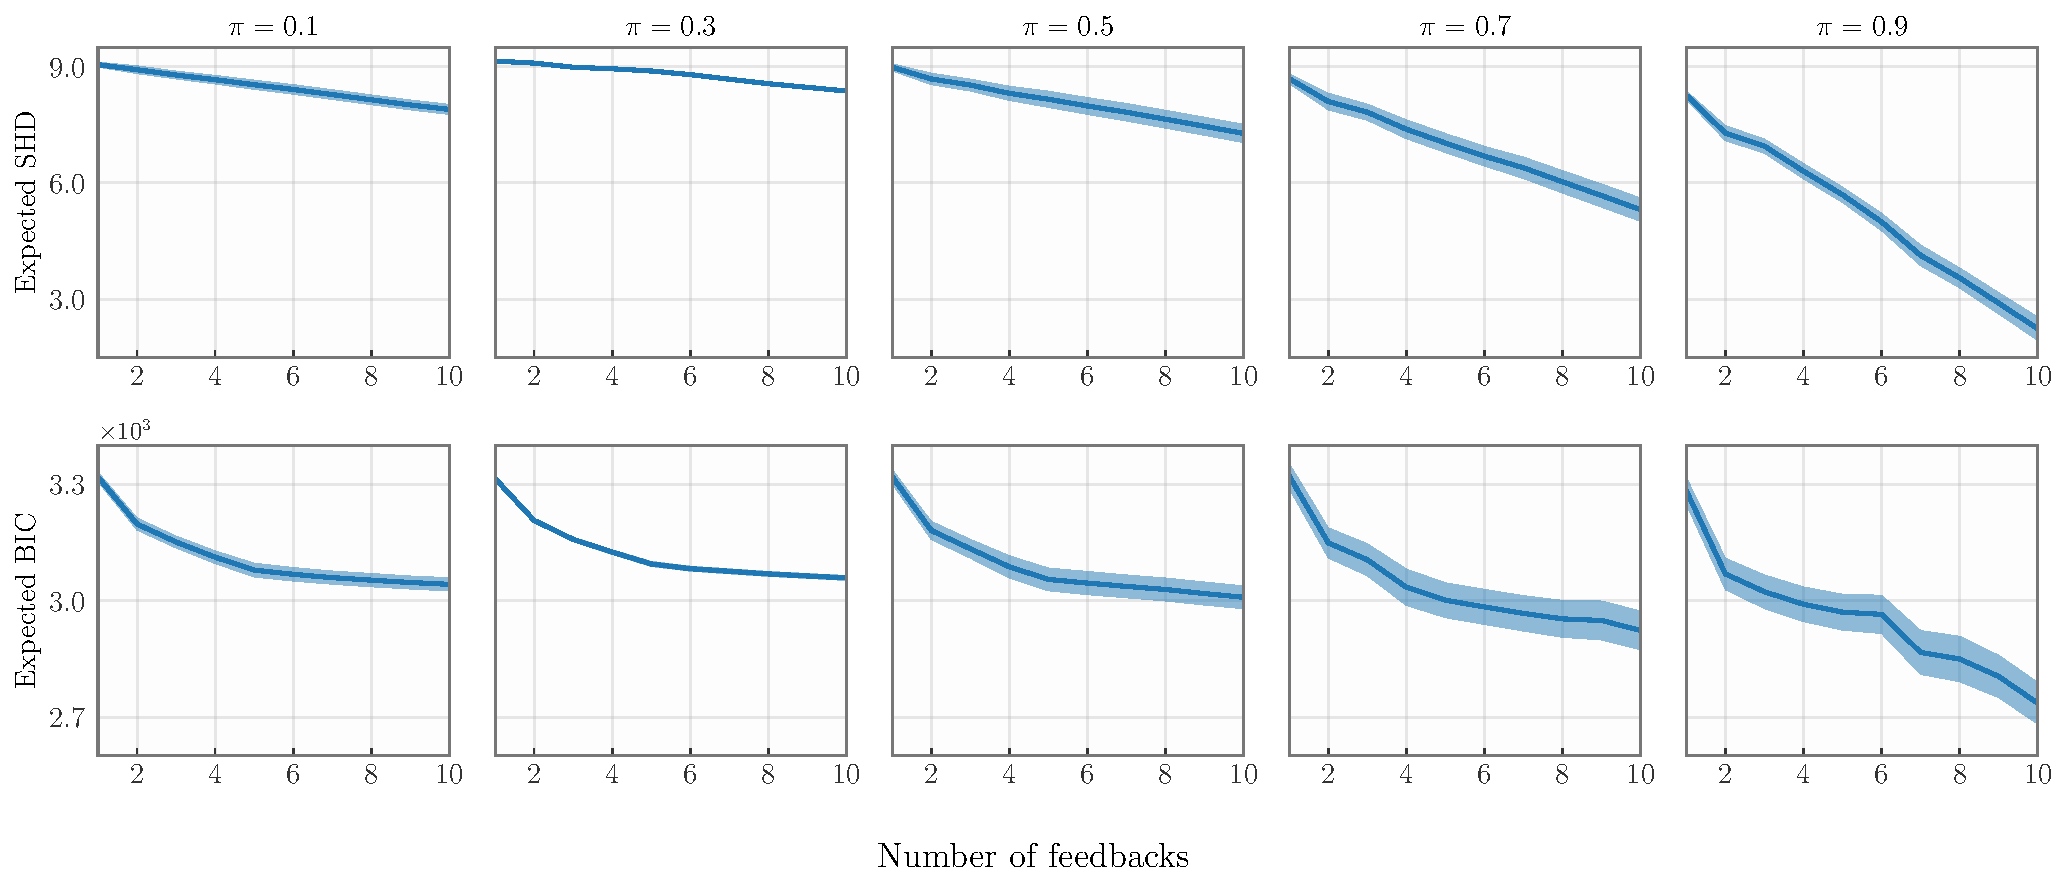
\includegraphics[width=\textwidth]{figures/hitl_sensibility.pdf} 
    \caption{\textbf{Sensitivity of our active knowledge elicitation framework to the reliability of the expert.} Each column represents either the expected SHD (top) or expected BIC (bottom) as a function of the degree of confidence $\pi \in [0, 1]$ in the expert as a function of the number of feedbacks. As expected, the improvements entailed by the expert's feedback become increasingly effective as we increase the expert's reliability from $0.1$ to $0.9$. Results reflect the outcome of 30 scenarios simulated accordingly to \cref{alg:hitl} with a random canonical diagram $\mathcal{G}^\star$ with $5$ nodes. We used our active knowledge elicitation scheme to select the query at each iteration.}
    \label{fig:feedbackspi}
\end{figure*}

\paragraph{Training hyperparameters.} For AGFN's forward flow, we use a Graph Isomorphism Network (GIN, \citet{DBLP:conf/iclr/XuHLJ19}) with $2$ layers to compute embeddings of dimension $256$. Then, we project these embeddings to a probability distribution using a three-layer MLP having leaky RELUs with a negative slope of $-0.01$ as activation functions. Correspondingly, we use an equally configured three-layer MLP to parametrize AGFN's backward flow. For training, we use the Adam method for the stochastic optimization problem defined by the minimization of the loss in \cref{eq:dbalancetheta}. Moreover, we trained the neural networks for $3000$ epochs for the human-in-the-loop simulations (in which we considered graphs having up to $10$ nodes) and for $500$ epochs for both the assessment of the distributional quality of AGFN and the comparison of AGFN with alternative CD approaches.  

\paragraph{Computational settings.} We trained the AGFNs for the experiments in \cref{fig:distribution} and \cref{tab:table} and \cref{fig:feedbacks} for $500$ epochs in computers equipped with NVIDIA's V100 GPUs. All the experiments were executed in a cluster of NVIDIA's V100 GPUs and the algorithms were implemented using the machine learning framework \texttt{PyTorch}. To estimate the PAG corresponding to AGFN's samples and compute the SHDs reported in \cref{tab:table}, we used the FCI's implementation of the \texttt{pcalg} package in \texttt{R} considering the d-separations entailed by these samples as a criterion for conditional dependence. 

% \noindent\textbf{BIC as a sparsity-inducing prior.} 

% \begin{enumerate}
%     \item Architectural choices, epochs. 
%     \item Practical guidelines for masking. 
% \end{enumerate}

\subsection{Human in the loop} \label{sec::hitl} 

\begin{algorithm}[t] 
    \caption{Simulating humans in the loop}\label{alg:hitl}
    \begin{algorithmic}
    \Require $\{\mathcal{G}_{t}\}_{1 \le t \le T} \text{ samples from AGFN}$, $\mathcal{G}^{*} = (\mathbf{V}, E)$ true ancestral graph, $\pi$ reliability of the expert's feedback 
    \State $p(\omega_r=k) \gets \frac{1}{T} \sum_{1 \le t \le T} 1_{\{\omega_r=k \text{ in } G_{t}\}} \forall k \in [4], r \in {\mathbf{V} \choose 2}$ 

    \State $\mathbf{f} \gets \{\}$ \Comment{Set of feedbacks (answers)} 
    \State $\boldsymbol{r} \gets \{\}$ \Comment{Set of queries (questions)} 

    \State $K \gets 1$

    \State $\omega_{r}^{*} \gets \text{ relation } r\text{'s feature in } \mathcal{G}^{*} \ \forall r \in {\mathbf{V} \choose 2}$  
    \While{$\boldsymbol{r} \neq {\mathbf{V} \choose 2}$}
        \Comment{Iteratively request the feedback}  
        \State $r_{K} \gets \underset{r \in {\mathbf{V} \choose 2} \setminus \boldsymbol{r}}{\argmax} \ \underset{{f_r \sim p(\cdot)}}{\mathbb{E}}[ -\mathbf{H} \left( q(\mathcal{G}; \mathbf{f} \cup \{f_r\}), q(\mathcal{G} ; \mathbf{f}) \right)]$ 
        \State $\mathbf{r} \gets \mathbf{r} \cup \{r_{K}\}$
        \State $f_{K} \sim \text{Cat}\left( \pi \cdot \delta_{\omega_{r_{K}}^{*}} + \left(\frac{1 - \pi}{3}\right) \cdot (1 - \delta_{\omega_{r_{K}}^{*}}) \right)$     
        \State $\mathbf{f} \gets \mathbf{f} \cup \{f_{K}\}$ 
        \State $K \gets K + 1$ 
    \EndWhile 
    \end{algorithmic}
\end{algorithm}

\paragraph{Algorithmic details.} We describe in \cref{alg:hitl} our procedure for simulating interactions with an expert. Initially, we estimate the marginal probabilities $p(\omega_{r}=k)$ of a relation $r$ displaying the feature $k \in \{1, 2, 3, 4\}$ under AGFN's learned distribution. This is our prior distribution. In \cref{alg:hitl}, we denote $\{1, 2, 3, 4\}$ by $[4]$. Then, we iteratively select the relation that maximizes our acquisition function; the simulated human thus returns a feedback that equals the selected relation's true feature with probability $\pi$ or is otherwise uniformly distributed among the incorrect alternatives. Importantly, this iterative mechanism can be interrupted at any iteration and the collected feedbacks can be used to compute the importance weights necessary for estimating expectations of functionals under our updated beliefs. 

% Importantly, this iterative mechanism could be interrupted at any iteration and the collected feedbacks could be used to compute the importance weights necessary for estimating expectations of functionals under our updated beliefs. 

\section{Additional experiments} 

\begin{figure}[!t] 
    \centering
    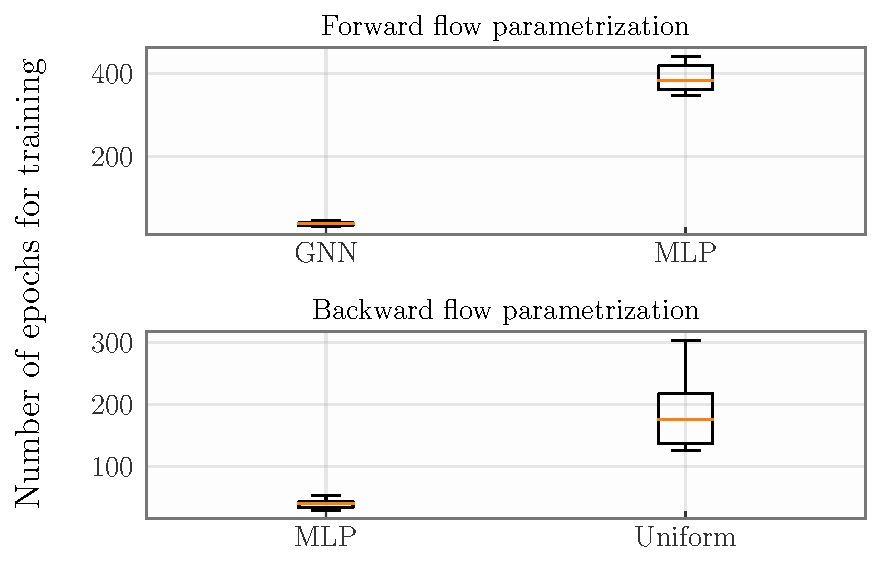
\includegraphics[width=.7\linewidth]{figures/ablations_arch.pdf} 
    \caption{\textbf{Architectural design of AGFN.} Top: The inductively biased parametrization of AGFN's forward flow --- based upon a GNN --- enables the substantial reduction of the number of epochs required for training. Bottom: The use of a parametrized backward policy similarly enhances the training efficiency compared to a uniform policy. For both experiments, we considered $\mathcal{L}(\theta) < 0.1$ as the early stopping criterion to interrupt AGFN's training.}
    \label{fig:arch}
\end{figure}

\paragraph{Trade-off between diversity and optimality in AGFN.} We may use tempered rewards to increase the frequency of high-scoring samples and thereby reduce the diversity of AGFN's distribution. More precisely, we choose a temperature $T$ and consider  
\begin{equation} \label{eq:tempering} 
    R_{T}(\mathcal{G}) = R(\mathcal{G})^{1/T} = \exp\left\{\frac{\mu - U(\mathcal{G})}{T \sigma}\right\} 
\end{equation}
as the reward upon which the GFlowNet is trained; if $T \rightarrow 0$, the distribution $p_{T} \propto R_{T}$ converges to a point mass in $R(\mathcal{G})$'s mode and, if $T \rightarrow \infty$, $p_{T}$ converges to an uniform distribution. This approach resembles the simulated tempering scheme commonly exploited in Monte Carlo methods \cite{parisi1992simulated} and was previously considered in the context of GFlowNets by \citet{zhang2023robust}. \Cref{fig:tempering} shows that progressively cold distributions (i.e., with $T \rightarrow 0$) lead to progressively concentrated and decreasingly diverse samples. Notably, the use of cold distributions may be adequate if we are highly confident in our score and are mostly interested in high-scoring samples  \cite[e.g., as in][]{DBLP:conf/uai/RantanenHJ21}. 

\begin{figure*}[!t] 
    \centering
    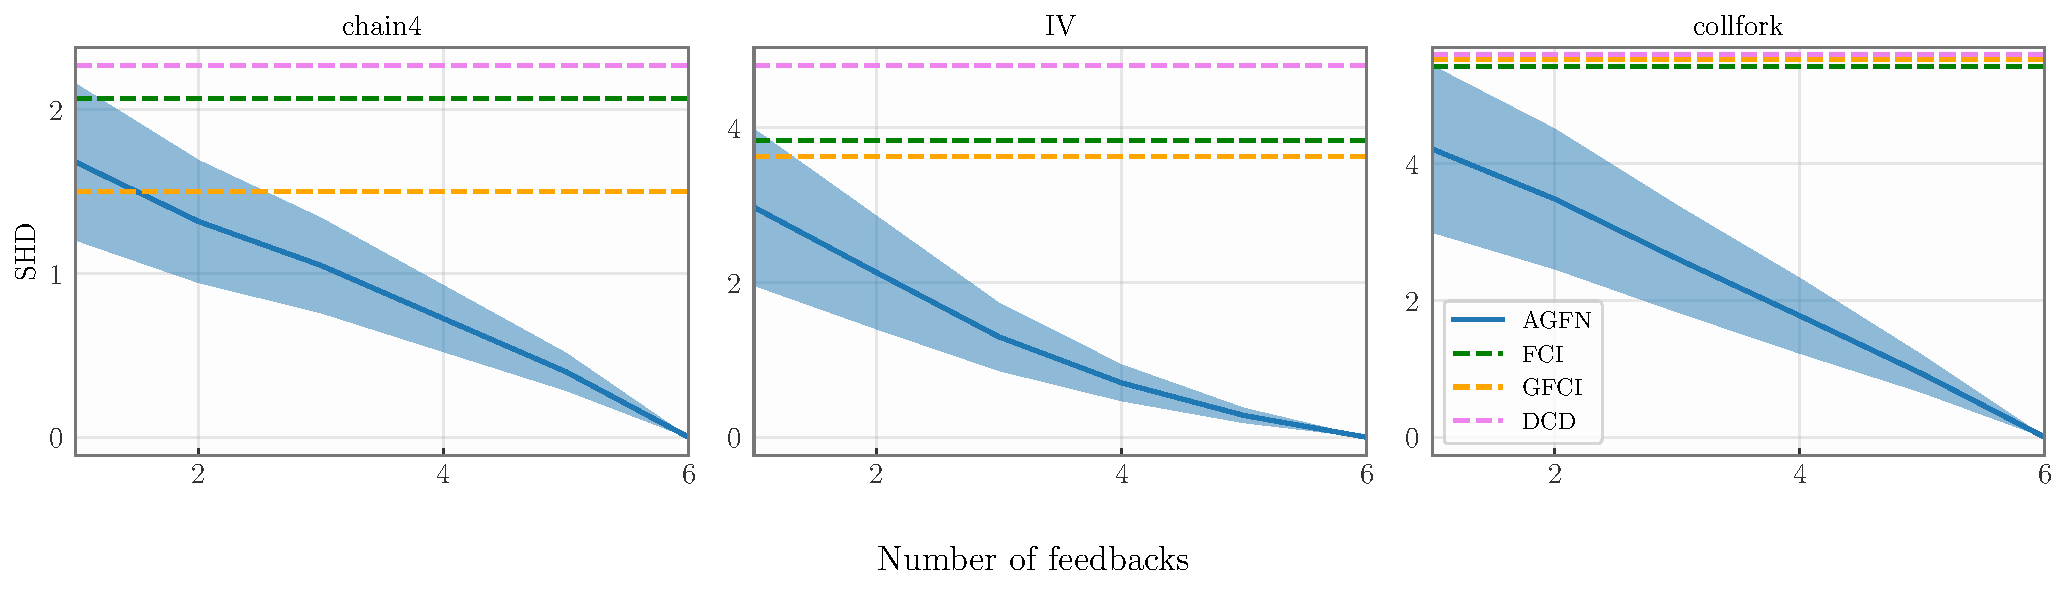
\includegraphics[width=\textwidth]{figures/hitl_benchmarks.pdf} 
    \caption{\textbf{Human-aided AGFN significantly outperforms alternative CD algorithms.} Updating AGFN's distribution according to the feedback of an oracle substantially improves AGFN's capacity to correctly identify the true ancestral graph; indeed, a single feedback is sufficient to yield results better than (or indistinguishable from) alternative CD algorithms. We select the sampled AG with the highest posterior reward as a point estimate of AGFN and use the same datasets listed in \cref{tab:tablee}. The plots summarize the results of $30$ HITL simulations using $\pi = 0.9$ and an oracle as an expert (see \cref{alg:hitl}).}
    \label{fig:tablehitl}
\end{figure*}

\paragraph{Sensitivity analysis for different noise levels.} \Cref{fig:feedbackspi} displays the effect of the feedback of an increasingly reliable expert over the expectations of both the SHD and the BIC. Notably, the usefulness of these feedbacks increases as the feedback noise decreases. This is expected as, for example, a completely unreliable expert consistently rules out only one of four possibilities for the features of each relation; then, there remains a great ambiguity, albeit not as much as there was prior to their feedback, about the true nature of the elicited causal relation. Moreover, this experiment highlights the potential to adjust the reliability parameter $\pi$ to incorporate knowledge into AGFN's learned distribution regarding the non-existence of a particular relation, rather than its existence. More specifically, assume that the expert is certain that there is no directed edge from the variable $U$ to the variable $V$ in the underlying ancestral graph; for instance, a doctor may be certain that cancer ($U$) is not an ancestor (cause) of smoking ($V$), but may be uncertain about the definite relation between $U$ and $V$ (i.e., smoking may or may not cause cancer). 
To incorporate such knowledge into our model, one approach is to set a necessarily small reliability parameter $\pi$ (possibly, $\pi = 0$) along with the improbable relation $U \rightarrow V$. This feedback will then be modeled as a relation unlikely to exist in the true ancestral graph. 
%elicit the expert's feedback about the relation 
%we may set $\pi = 0$ and elicit the expert's feedback about the causal relation between the variables $U$ and $V$ (in the previous example, if $U$ represents cancer and $V$ represents smoking, the expert may provide a feedback $U \rightarrow V$ with a small reliability parameter, meaning that this relation is unlikely to exist in the true ancestral graph). 
We emphasize that our model for the expert's responses is straightforwardly extensible to accommodate multiple feedbacks about the same causal relation under different reliability levels. % \textcolor{red}{Especificar qual GNN usamos}   

\paragraph{Ablation studies.} \Cref{fig:arch} shows the increase in the training efficiency due to our architectural designs for parametrizing both the forward and backward flows of AGFN. Noticeably, the use of a two-layer graph isomorphism network \cite[GIN;][]{DBLP:conf/iclr/XuHLJ19} with a 256-dimensional embedding for the forward flow entailed a decrease of more than 10x in the number of epochs required for successfully training AGFN; this highlights the effectiveness of an inductively biased architectural design for the parametrization of GFlowNet's flows. Correlatively, the use of a parametrized backward flow significantly enhances the training efficiency of AGFN and emphasizes the inadequacy of a uniformly distributed backward policy pointed out in a previous work \cite{shen2023towards}.  

\paragraph{Human-aided AGFN versus alternative CD methods.} \Cref{fig:tablehitl} exposes the significant enhancement of AGFN's point estimates entailed by our HITL framework for CD. 
This underlines the usefulness of the elicited knowledge, which is simply incorporated into our model through a re-weighting of the reward function, enabling the identification of the true ancestral graph. In contrast, most alternative CD algorithms cannot be as easily adapted to include various forms of expert knowledge --- and such incorporation, when it is possible, usually precedes any inferential process \cite{DBLP:conf/aistats/Andrews20} or assumes the knowledge is perfect \cite{DBLP:conf/nips/WangQZ22}. % , thus blinding the expert about the latent weaknesses of the inferential process.  

% which blinds the expert about the latent weaknesses of the method and substantially difficult the affair of providing an informative feedback. 
% Importantly, we considered here that the expert is an oracle that consistently provides the correct causal relation between a pair of variables. 

% We measure the sensibility of our approach to the level of noiseness of the expert. 

% My plan is to report 

% \begin{enumerate}
%     \item a figure similar to \cref{fig:feedbacks} representing the improvement enacted by the expert's feedback on AGFN's distribution, and 
%     \item a table with the average relative improvements over the considered metrics with respect to the individually unsupervised distribution.  
% \end{enumerate}

% Moreover, I should prepare the code and start with the experiments for real-world datasets. 
% \bibliography{aaai24} 
% \section{Additional results}

% \begin{enumerate}
%     \item Algorithmic details. 
%     \item Sensibility analysis. 
% \end{enumerate}


\bibliographystyle{plainnat} 
\bibliography{aaai24} 

\end{document}
